%%%%%%%%%%%%%%%%%%%%%%%%%%%%%%%%%%%%%%%%%%%%%%%%%%%%%%%%%%%%%%%%%%%%%%%%%%%%%%%%
\begin{frame}[fragile]\frametitle{}
\begin{center}
{\Large Conclusion}
\end{center}
\end{frame}

%%%%%%%%%%%%%%%%%%%%%%%%%%%%%%%%%%%%%%%%%%%%%%%%%%%%%%%%%%%
\begin{frame}[fragile]\frametitle{Transformer Overview}

\begin{columns}
    \begin{column}[T]{0.5\linewidth}
			\begin{center}
			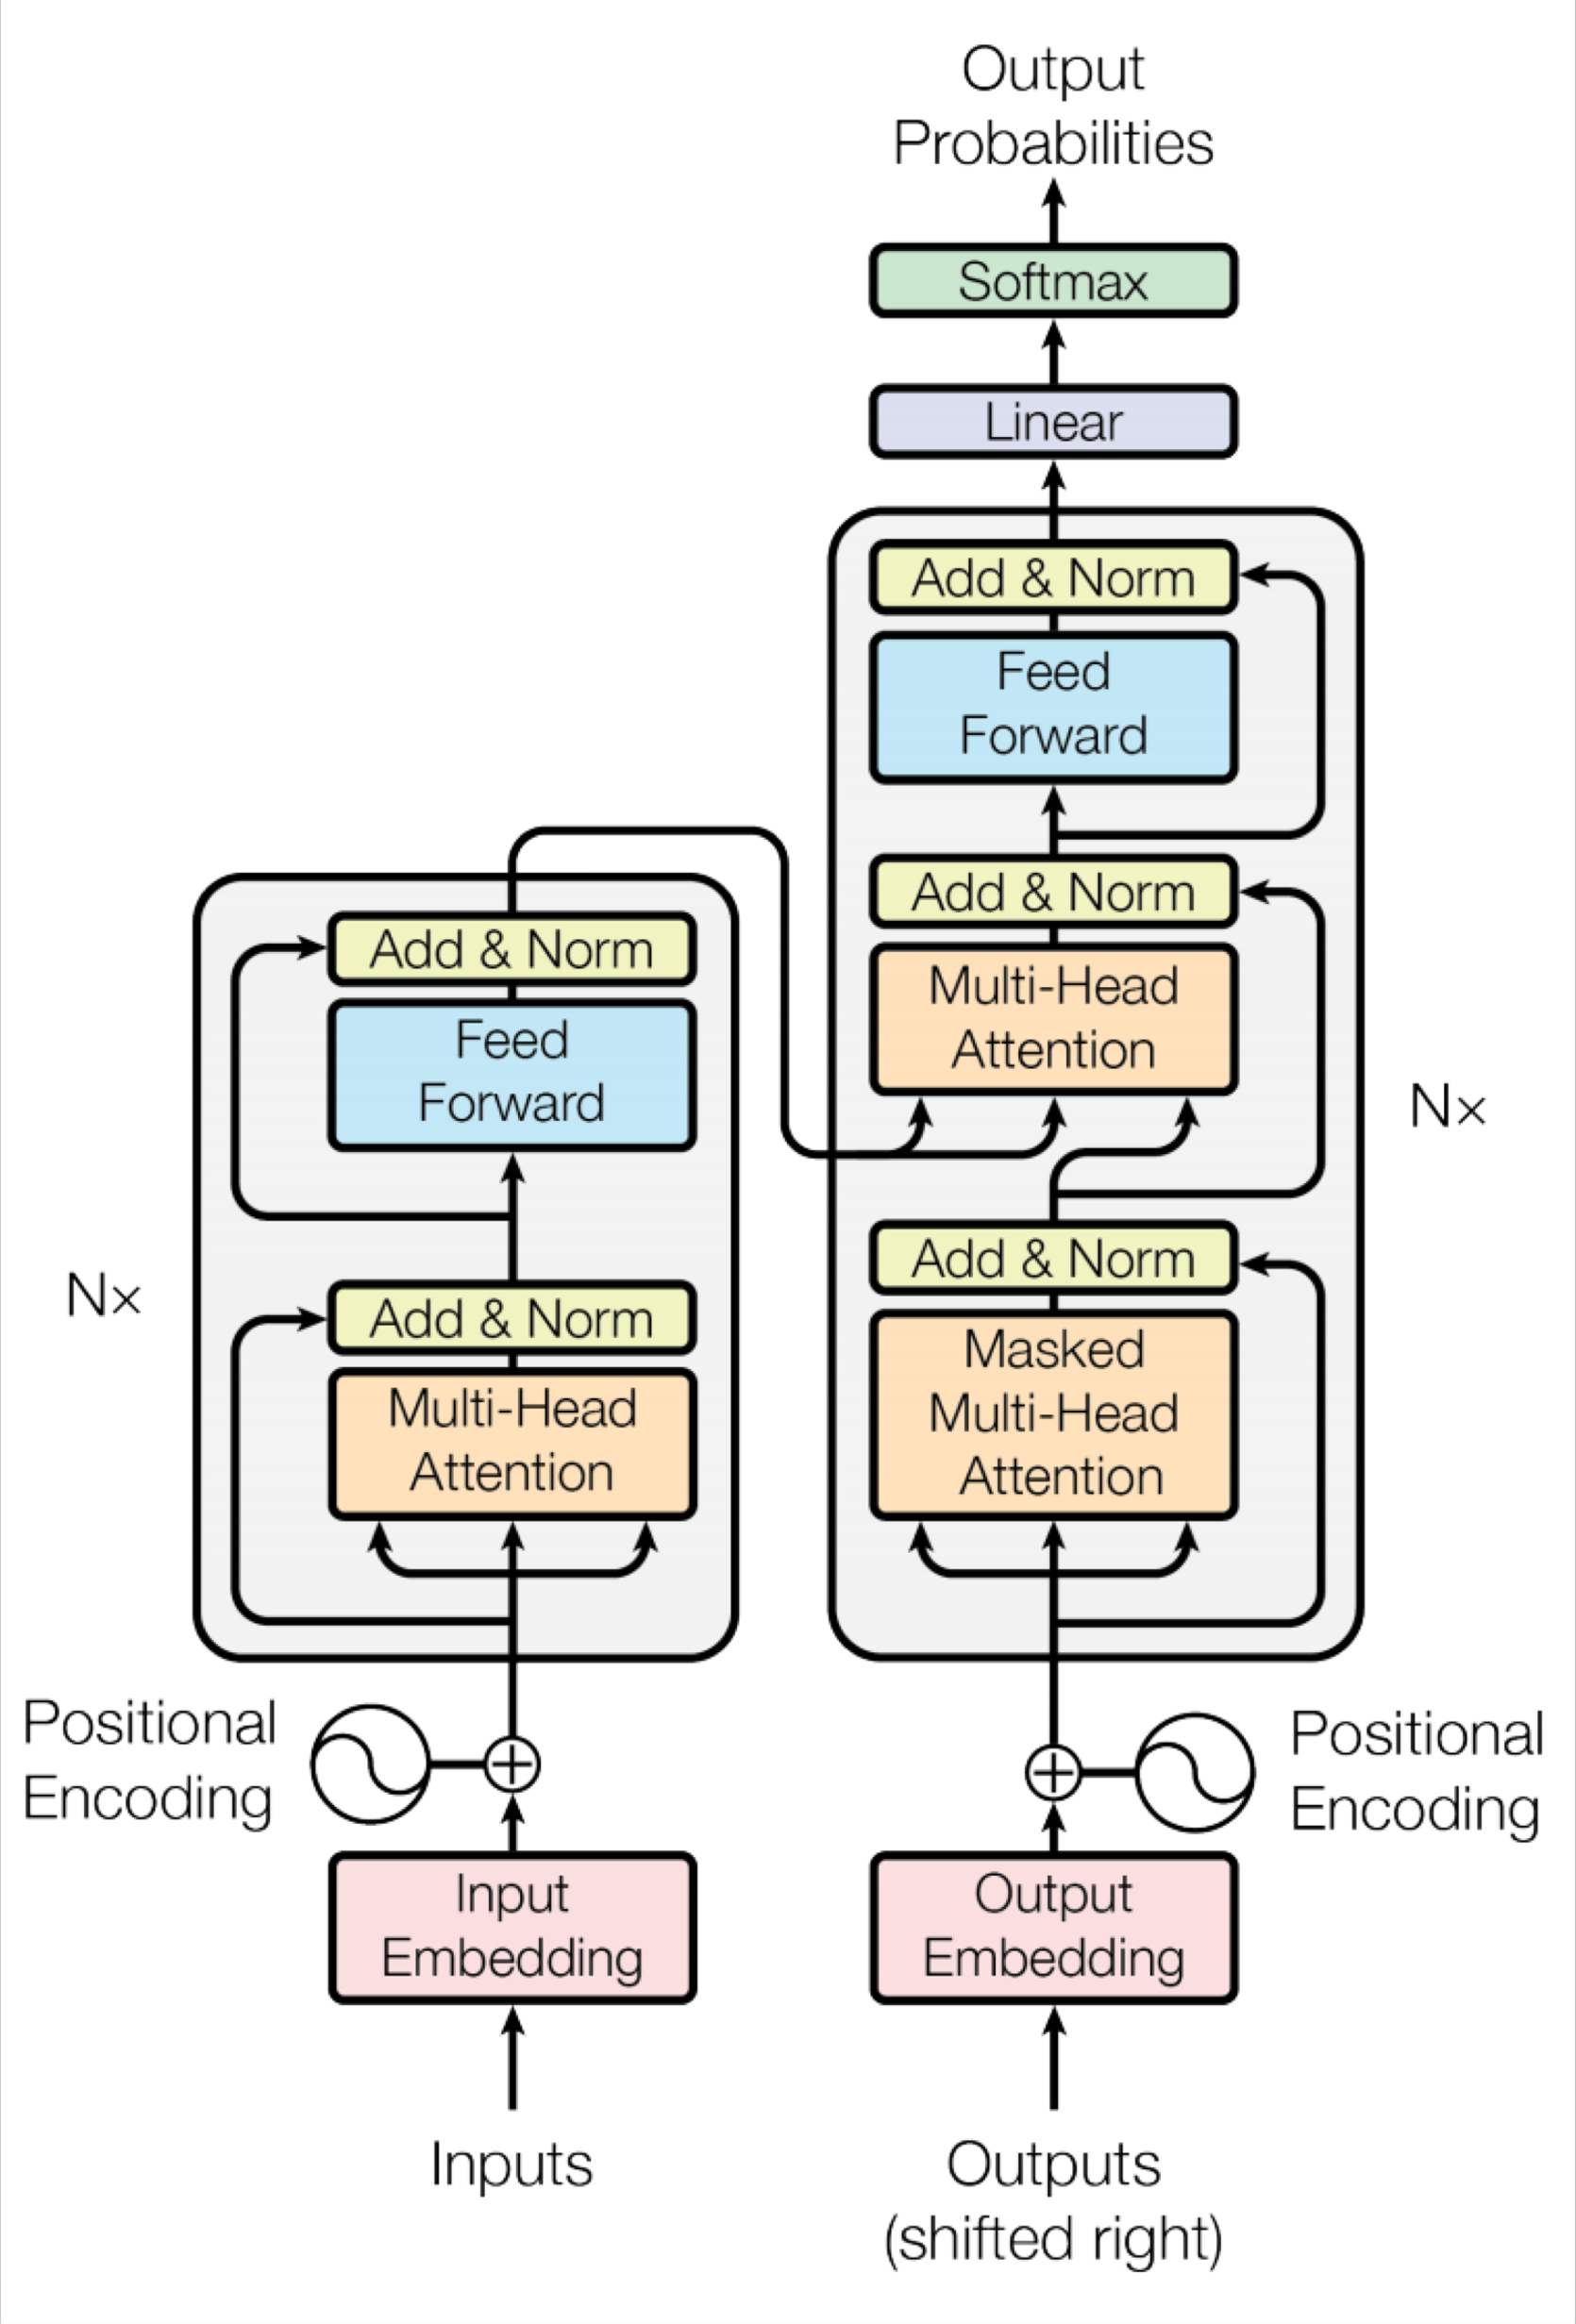
\includegraphics[width=0.8\linewidth,keepaspectratio]{bert69}
			\end{center}		
		\end{column}
    \begin{column}[T]{0.5\linewidth}
		Attention is all you need. 2017.  Aswani, Shazeer, Parmar, Uszkoreit,  Jones, Gomez, Kaiser, Polosukhin  https://arxiv.org/pdf/1706.03762.pdf 

      \begin{itemize}
			\item Non-recurrent sequence-to-  sequence encoder-decoder model
			\item Task: machine translation  with parallel corpus
			\item Predict each translated word
			\item Final cost/error function is  standard cross-entropy error on top of a softmax classifier
			\end{itemize}
    \end{column}
  \end{columns}
			
\end{frame}

%%%%%%%%%%%%%%%%%%%%%%%%%%%%%%%%%%%%%%%%%%%%%%%%%%%%%%%%%%%
\begin{frame}[fragile]\frametitle{Architecture}

\begin{columns}
    \begin{column}[T]{0.5\linewidth}
			\begin{center}
			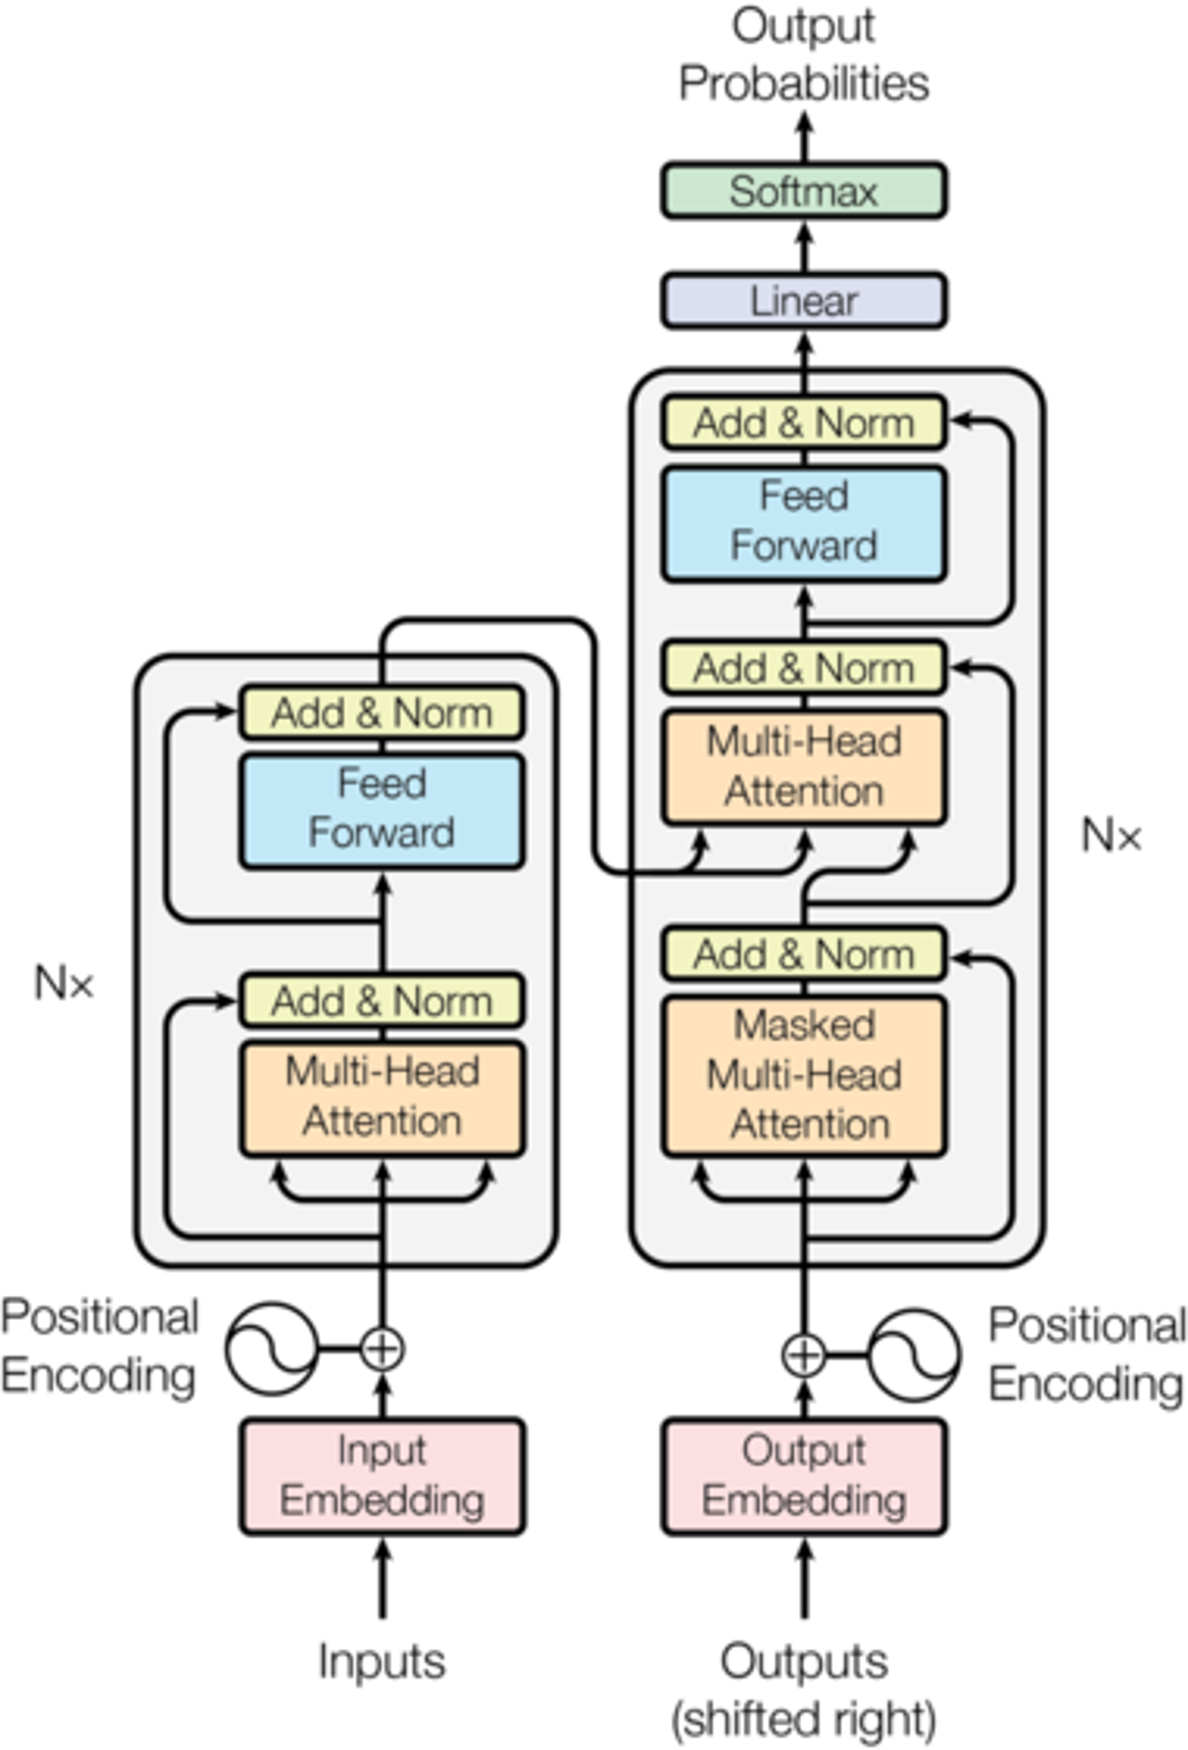
\includegraphics[width=0.8\linewidth,keepaspectratio]{bert65}
			\end{center}		
		\end{column}
    \begin{column}[T]{0.5\linewidth}
      \begin{itemize}
			\item Encoder-Decoder was there
			\item New?: Multi head attention
			\item Fine tuned with Custom Data
			\item Flavors:
      \begin{itemize}
			\item Encoder only
			\item Decoder only
			\item Encoder-Decoder
			\end{itemize}
			\end{itemize}
    \end{column}
  \end{columns}
			
\end{frame}


% %%%%%%%%%%%%%%%%%%%%%%%%%%%%%%%%%%%%%%%%%%%%%%%%%%%%%%%%%%%
% \begin{frame}[fragile]\frametitle{Transformer Encoder}

% \begin{columns}
    % \begin{column}[T]{0.5\linewidth}
			% \begin{center}
			% 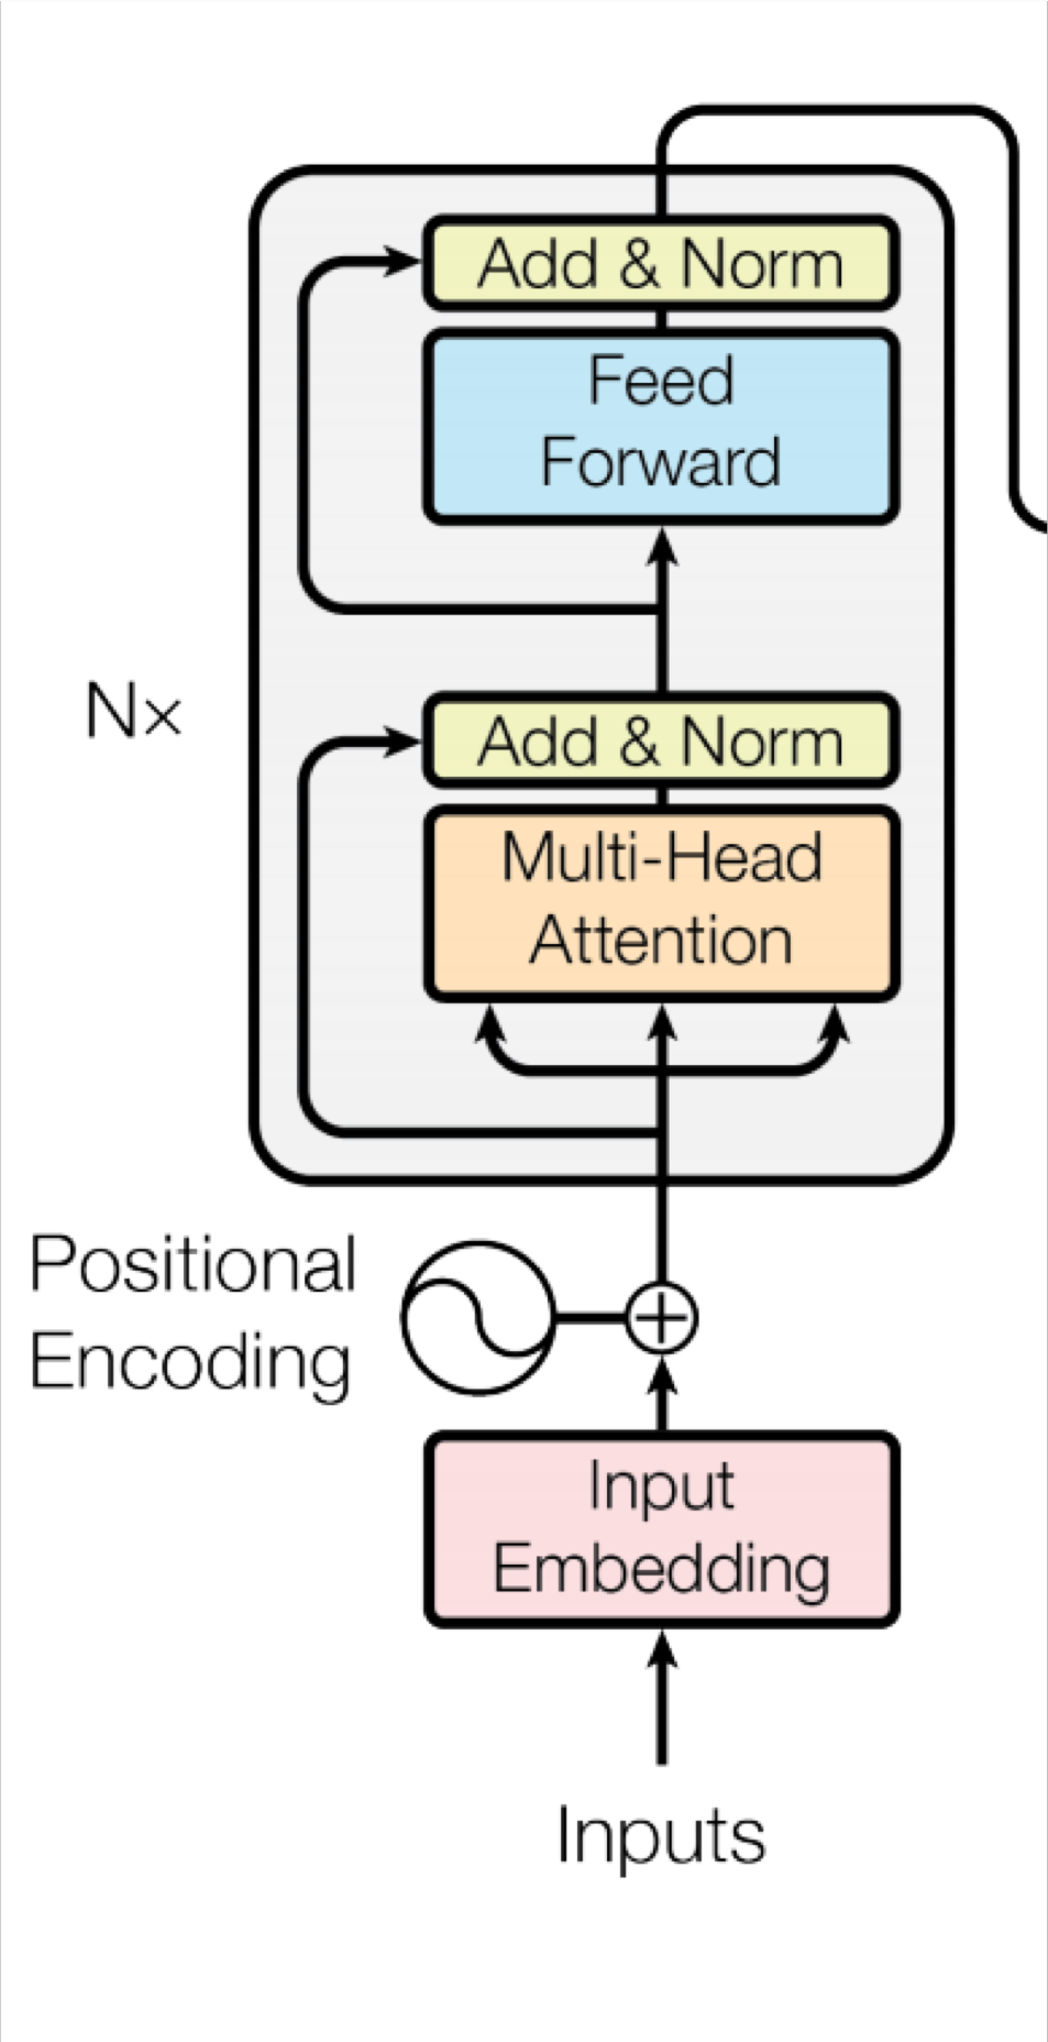
\includegraphics[width=0.6\linewidth,keepaspectratio]{bert70}
			% \end{center}		
		% \end{column}
    % \begin{column}[T]{0.5\linewidth}
      % \begin{itemize}
			% \item For encoder, at each block, we use the same Q, K and V; from the previous layer
			% \item Blocks are repeated 6 times (in vertical stack)
			% \end{itemize}
    % \end{column}
  % \end{columns}
			
% \end{frame}


%%%%%%%%%%%%%%%%%%%%%%%%%%%%%%%%%%%%%%%%%%%%%%%%%%%%%%%%%%%
\begin{frame}[fragile]\frametitle{Encoder only}

\begin{columns}
    \begin{column}[T]{0.5\linewidth}
			\begin{center}
			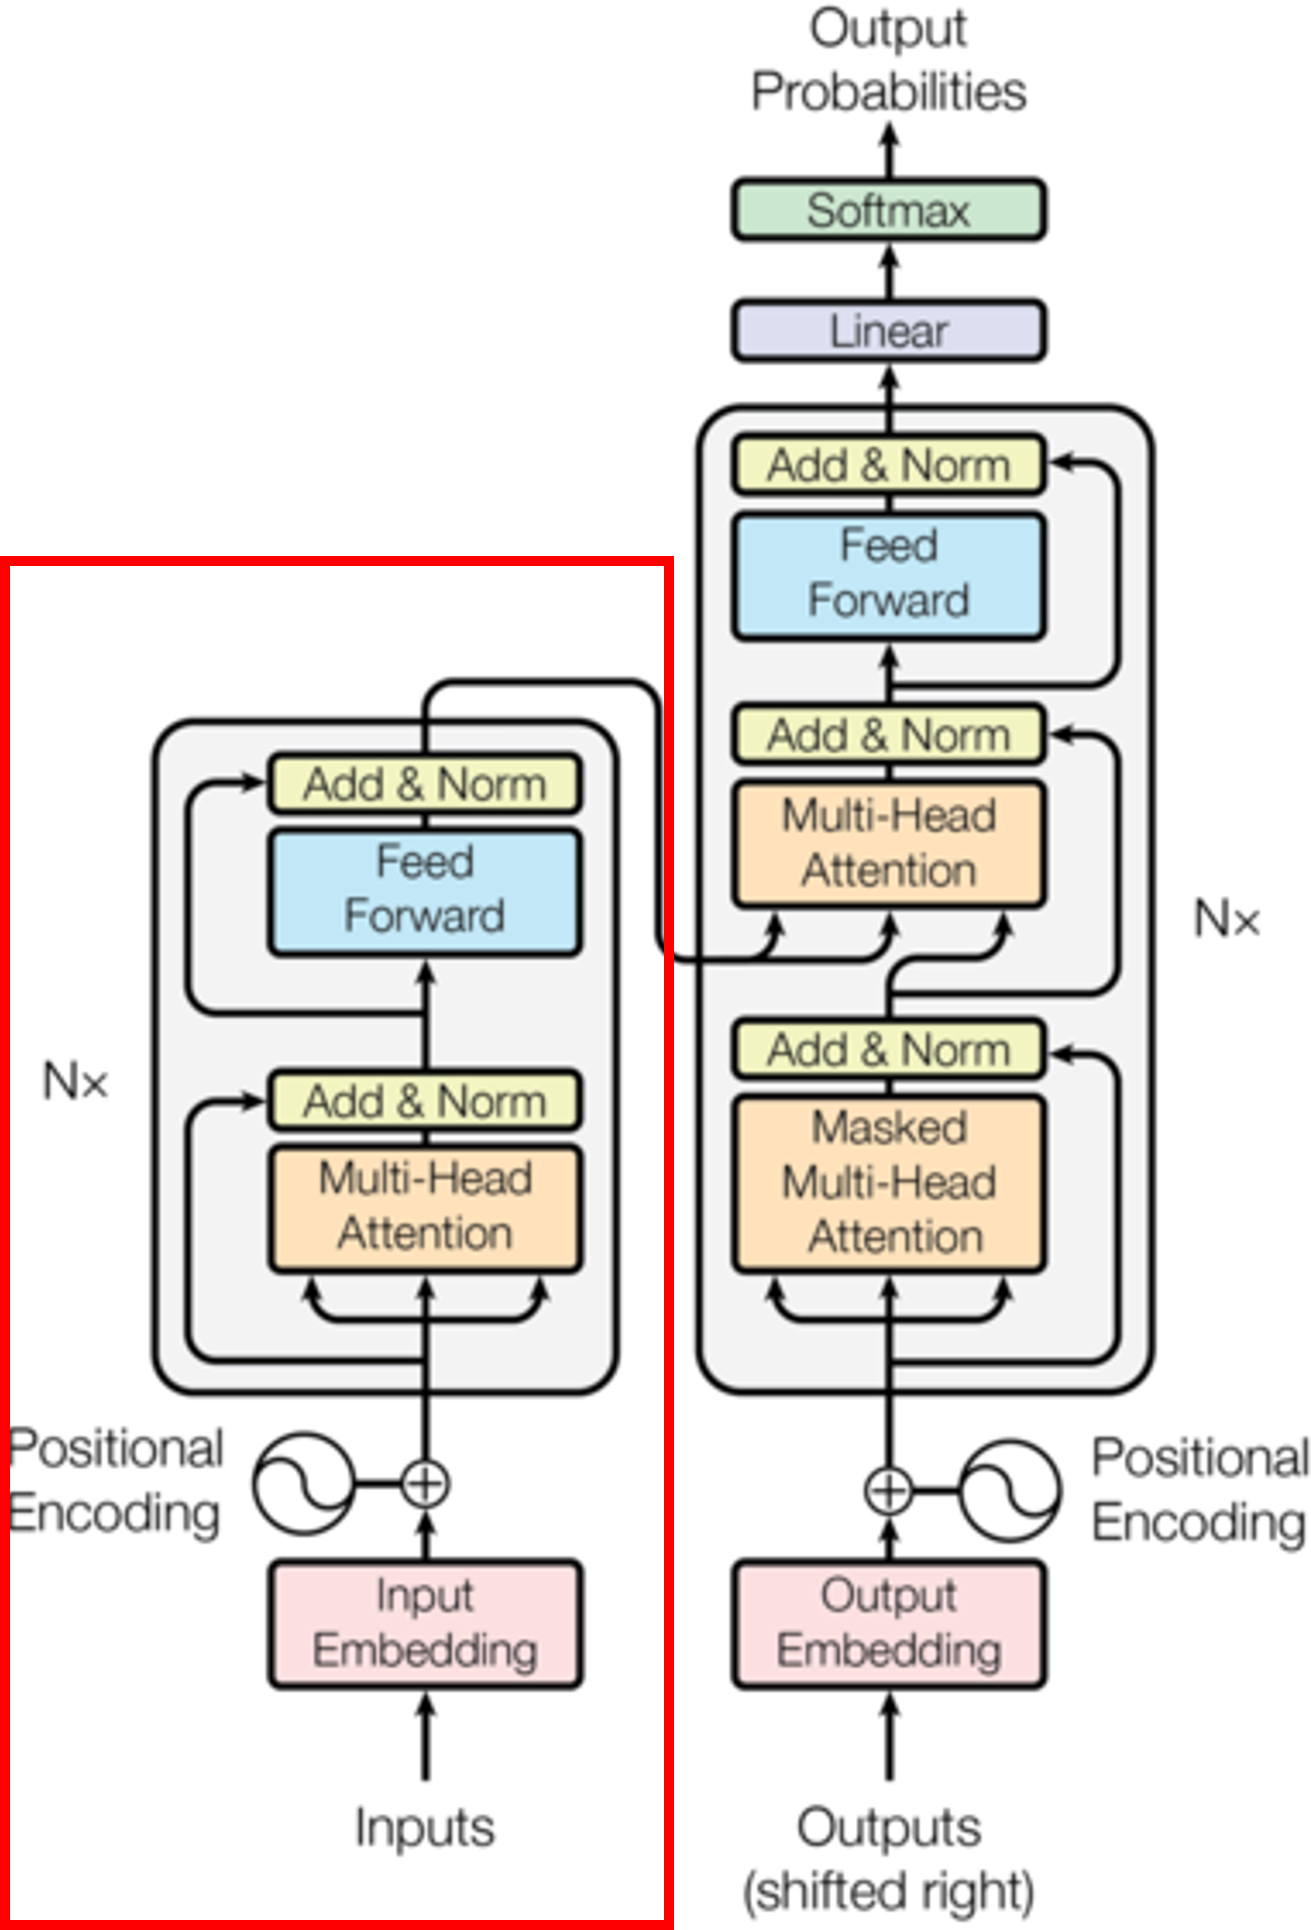
\includegraphics[width=0.8\linewidth,keepaspectratio]{bert66}
			\end{center}		
		\end{column}
    \begin{column}[T]{0.5\linewidth}
      \begin{itemize}
			\item If we are only interested in training a language model for the input for some other tasks, then we do not need the decoder of the transformer. 
			\item Pre-trained by predicting masked word
			\item BERT, XLNet, DistillBERT, RoBERTA
			\item Usage:
      \begin{itemize}
			\item Text Classification
			\item Named Entity Recognition
			\item Extractive Question Answering
			\end{itemize}
			\end{itemize}
    \end{column}
  \end{columns}
			
\end{frame}

% %%%%%%%%%%%%%%%%%%%%%%%%%%%%%%%%%%%%%%%%%%%%%%%%%%%%%%%%%%%
% \begin{frame}[fragile]\frametitle{Transformer Decoder}


			% \begin{center}
			% 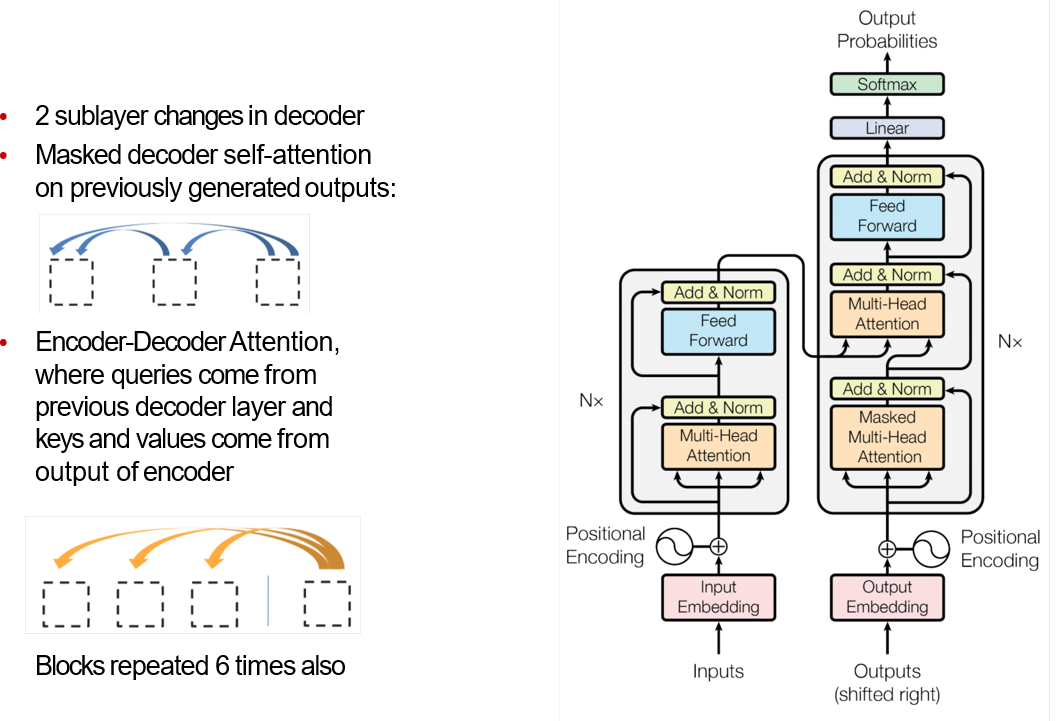
\includegraphics[width=\linewidth,keepaspectratio]{bert71}
			% \end{center}		

			
% \end{frame}


%%%%%%%%%%%%%%%%%%%%%%%%%%%%%%%%%%%%%%%%%%%%%%%%%%%%%%%%%%%
\begin{frame}[fragile]\frametitle{Decoder only}

\begin{columns}
    \begin{column}[T]{0.5\linewidth}
			\begin{center}
			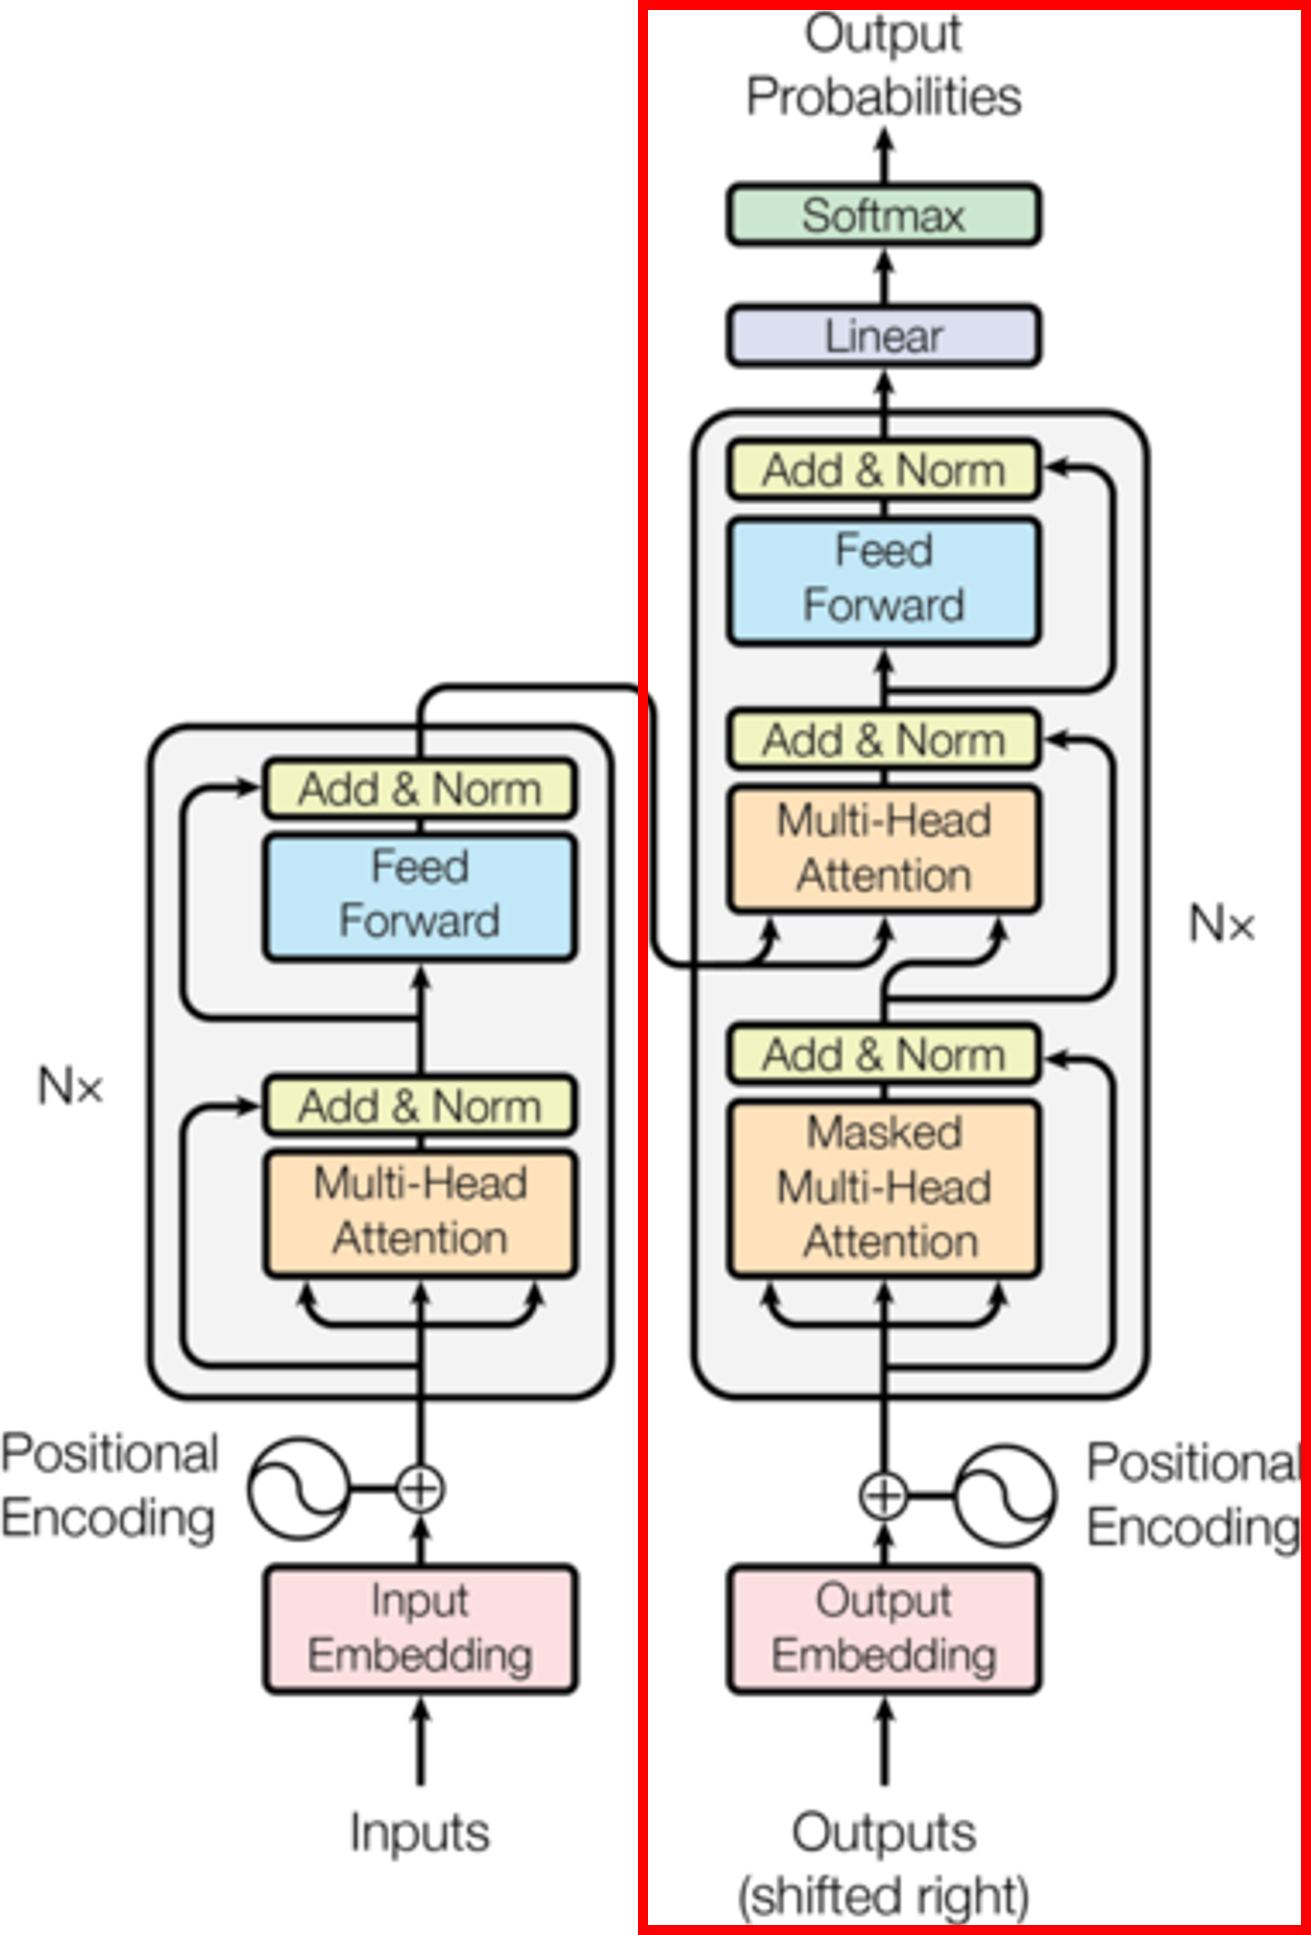
\includegraphics[width=0.8\linewidth,keepaspectratio]{bert67}
			\end{center}		
		\end{column}
    \begin{column}[T]{0.5\linewidth}
      \begin{itemize}
			\item If we do not have input, we just want to model the “next word”, we can get rid of the encoder side of a transformer and output “next word” one by one. 
			\item Pre-trained by predicting next word
			\item GPT-*, Transformer XL
			\item Usage:
      \begin{itemize}
			\item Text Generation
			\end{itemize}
			\end{itemize}
    \end{column}
  \end{columns}
			
\end{frame}


%%%%%%%%%%%%%%%%%%%%%%%%%%%%%%%%%%%%%%%%%%%%%%%%%%%%%%%%%%%
\begin{frame}[fragile]\frametitle{Encoder-Decoder, both}

\begin{columns}
    \begin{column}[T]{0.5\linewidth}
			\begin{center}
			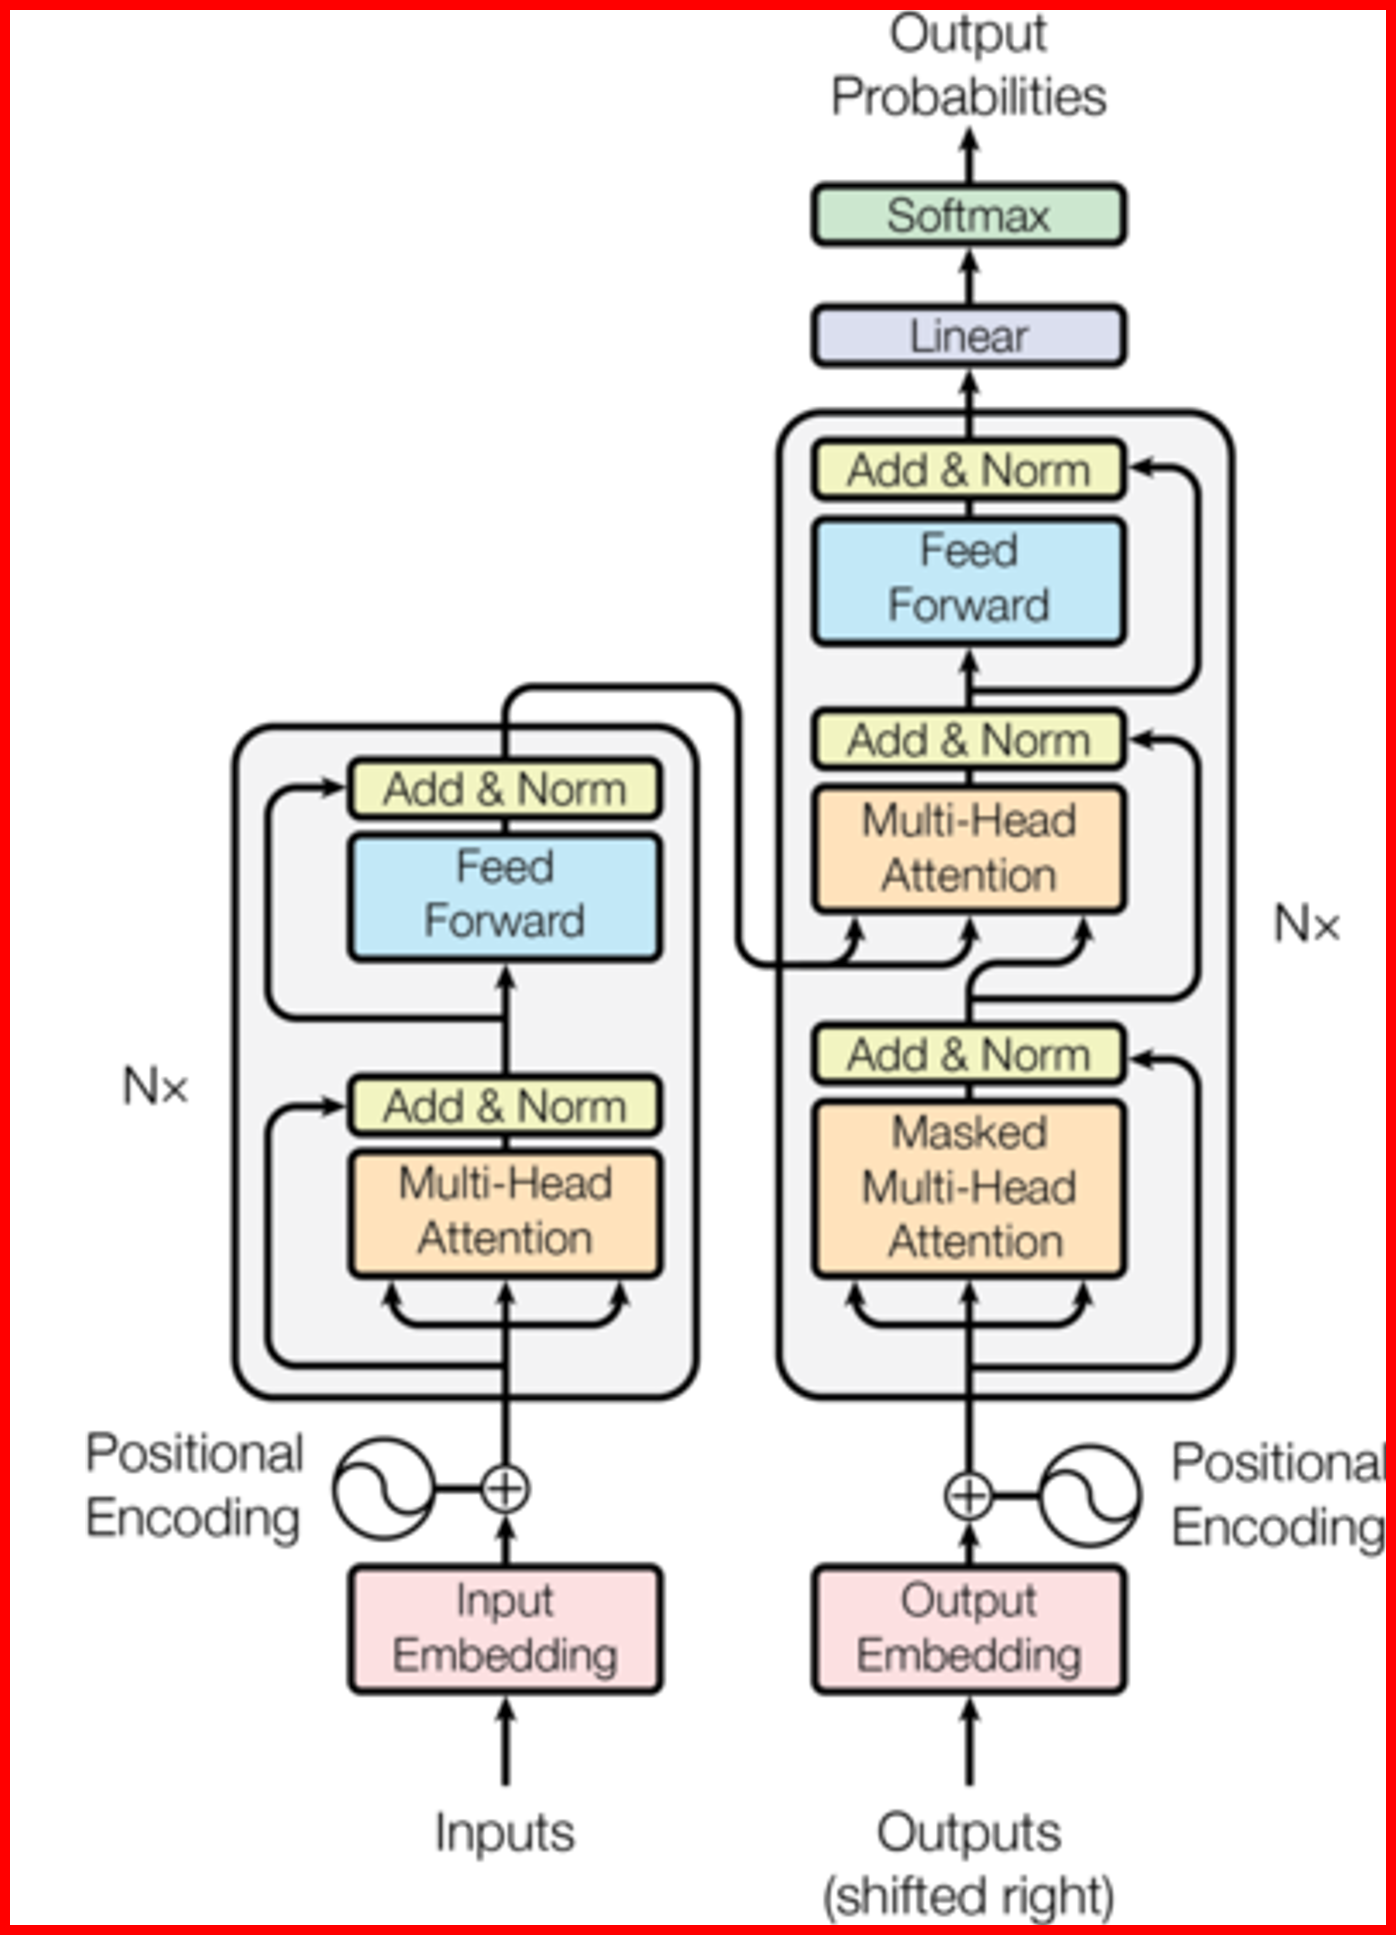
\includegraphics[width=0.8\linewidth,keepaspectratio]{bert68}
			\end{center}		
		\end{column}
    \begin{column}[T]{0.5\linewidth}
      \begin{itemize}
			\item Pre-trained by Seq2Seq manner
			\item T5, BART, PEGASUS
			\item Usage:
      \begin{itemize}
			\item Text summarization
			\item Machine Translation
			\item SQL generation
			\end{itemize}
			\end{itemize}
    \end{column}
  \end{columns}
			
\end{frame}

% %%%%%%%%%%%%%%%%%%%%%%%%%%%%%%%%%%%%%%%%%%%%%%%%%%%%%%%%%%%%%%%%%%%%%%%%%%%%%%%%%
% \begin{frame}[fragile]\frametitle{}
% \begin{center}
% {\Large Transformer \\ \small A quick tour}
% \end{center}
% \end{frame}


% %%%%%%%%%%%%%%%%%%%%%%%%%%%%%%%%%%%%%%%%%%%%%%%%%%%%%%%%%%%
% \begin{frame}[fragile]\frametitle{Transformers}


% \begin{itemize}
% \item The Transformer  is a model that uses attention to boost the speed with which seq2seq with attention models can be trained. The biggest benefit, however, comes from how The Transformer lends itself to parallelization. We will break it apart and look at how it functions.
% \item In its heart it contains an encoding component, a decoding component, and connections between them.
% \end{itemize}	 

% \begin{center}
% 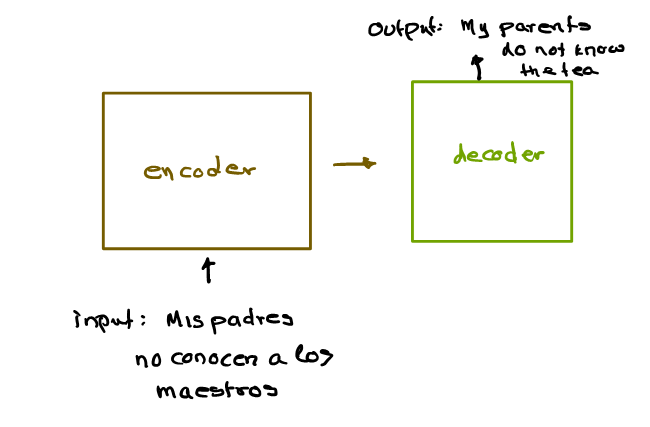
\includegraphics[width=0.6\linewidth,keepaspectratio]{bert51}
% \end{center}	

% \end{frame}


% %%%%%%%%%%%%%%%%%%%%%%%%%%%%%%%%%%%%%%%%%%%%%%%%%%%%%%%%%%%
% \begin{frame}[fragile]\frametitle{Transformers}
% \begin{columns}
    % \begin{column}[T]{0.5\linewidth}
      % \begin{itemize}
			% \item The encoding is a stack of encoders.
			% \item The original paper stacks six of them on top of each other – there’s nothing magical about the number six, one can definitely experiment with other arrangements). 
			% \item The decoding is a stack of decoders of the same number.
			% \end{itemize}
		% \end{column}
    % \begin{column}[T]{0.5\linewidth}
		
			% \begin{center}
			% 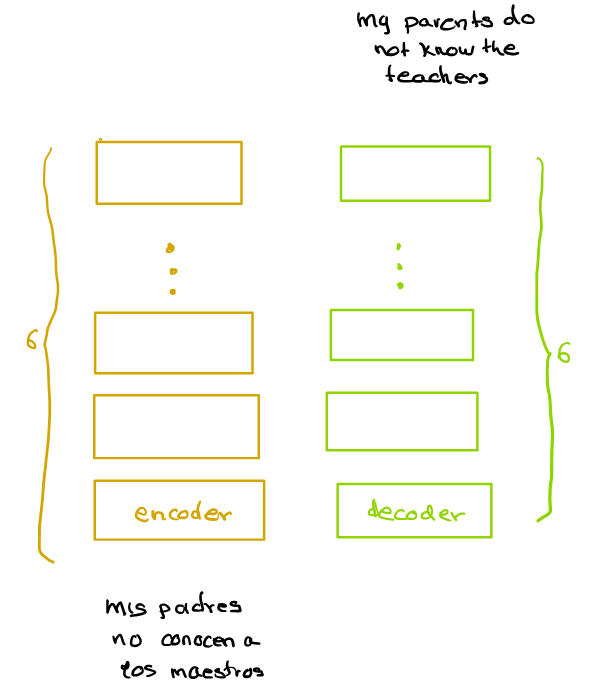
\includegraphics[width=0.8\linewidth,keepaspectratio]{bert52}
			% \end{center}

    % \end{column}
  % \end{columns}
% \end{frame}


% %%%%%%%%%%%%%%%%%%%%%%%%%%%%%%%%%%%%%%%%%%%%%%%%%%%%%%%%%%%
% \begin{frame}[fragile]\frametitle{Transformers}
% \begin{columns}
    % \begin{column}[T]{0.5\linewidth}
     % The encoder’s inputs goes through a self-attention layer – a layer that helps the encoder look at other words in the input sentence as it encodes a specific word.  
		% \end{column}
    % \begin{column}[T]{0.5\linewidth}
		% The decoder has both those layers, but between them is an attention layer that helps the decoder focus on relevant parts of the input sentence (similar what attention does in seq2seq models).
    % \end{column}
  % \end{columns}
	
			% \begin{center}
			% 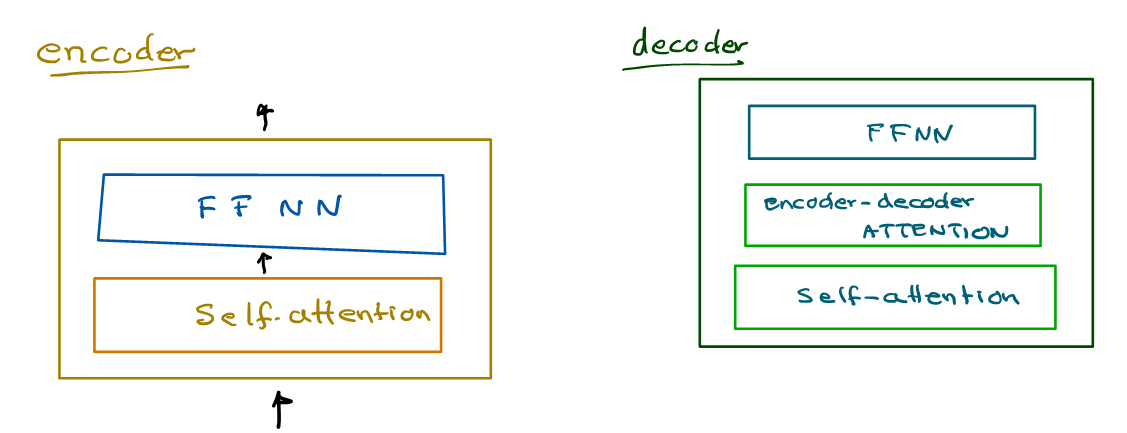
\includegraphics[width=0.8\linewidth,keepaspectratio]{bert53}
			% \end{center}
			
% \end{frame}

% %%%%%%%%%%%%%%%%%%%%%%%%%%%%%%%%%%%%%%%%%%%%%%%%%%%%%%%%%%%
% \begin{frame}[fragile]\frametitle{Transformers}
% \begin{columns}
    % \begin{column}[T]{0.5\linewidth}
			% \begin{center}
			% 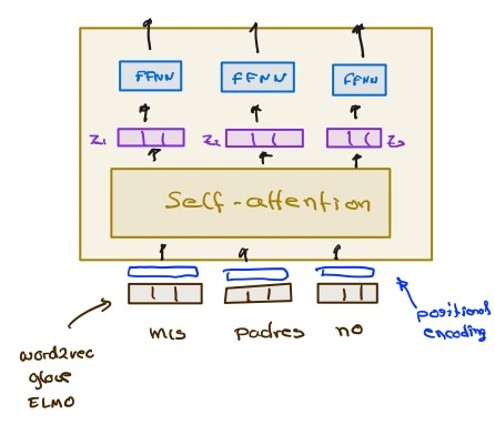
\includegraphics[width=0.8\linewidth,keepaspectratio]{bert58}
			% \end{center}		
		% \end{column}
    % \begin{column}[T]{0.5\linewidth}
      % \begin{itemize}
			% \item A key property of the Transformer, which is that the word in each position flows through its own path in the encoder. There are dependencies between these paths in the self-attention layer. 
			% \item The feed-forward layer does not have those dependencies, Therefore, the various paths can be executed in parallel while flowing through the feed-forward layer.
			% \end{itemize}
    % \end{column}
  % \end{columns}
			
% \end{frame}

% %%%%%%%%%%%%%%%%%%%%%%%%%%%%%%%%%%%%%%%%%%%%%%%%%%%%%%%%%%%
% \begin{frame}[fragile]\frametitle{Transformers}
% Patrick was not late for class because {\bf he} is a responsible student

% \begin{columns}
    % \begin{column}[T]{0.5\linewidth}
			% \begin{center}
			% 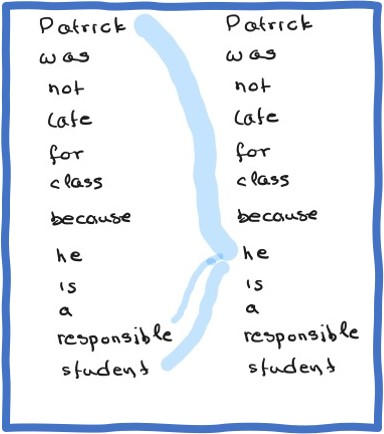
\includegraphics[width=\linewidth,keepaspectratio]{bert54}
			% \end{center}		
		% \end{column}
    % \begin{column}[T]{0.5\linewidth}
      % \begin{itemize}
			% \item What does ``he'' in this sentence refer to? Is it referring to the class or to the student? It's a simple question to a human, but not as simple to an algorithm.
			% \item When the model is processing the word ``he'', self-attention allows it to associate ``he'' with ``Patrick''.
			% \end{itemize}
    % \end{column}
  % \end{columns}
			
% \end{frame}

% %%%%%%%%%%%%%%%%%%%%%%%%%%%%%%%%%%%%%%%%%%%%%%%%%%%%%%%%%%%
% \begin{frame}[fragile]\frametitle{Transformers}
	% \begin{center}
	% 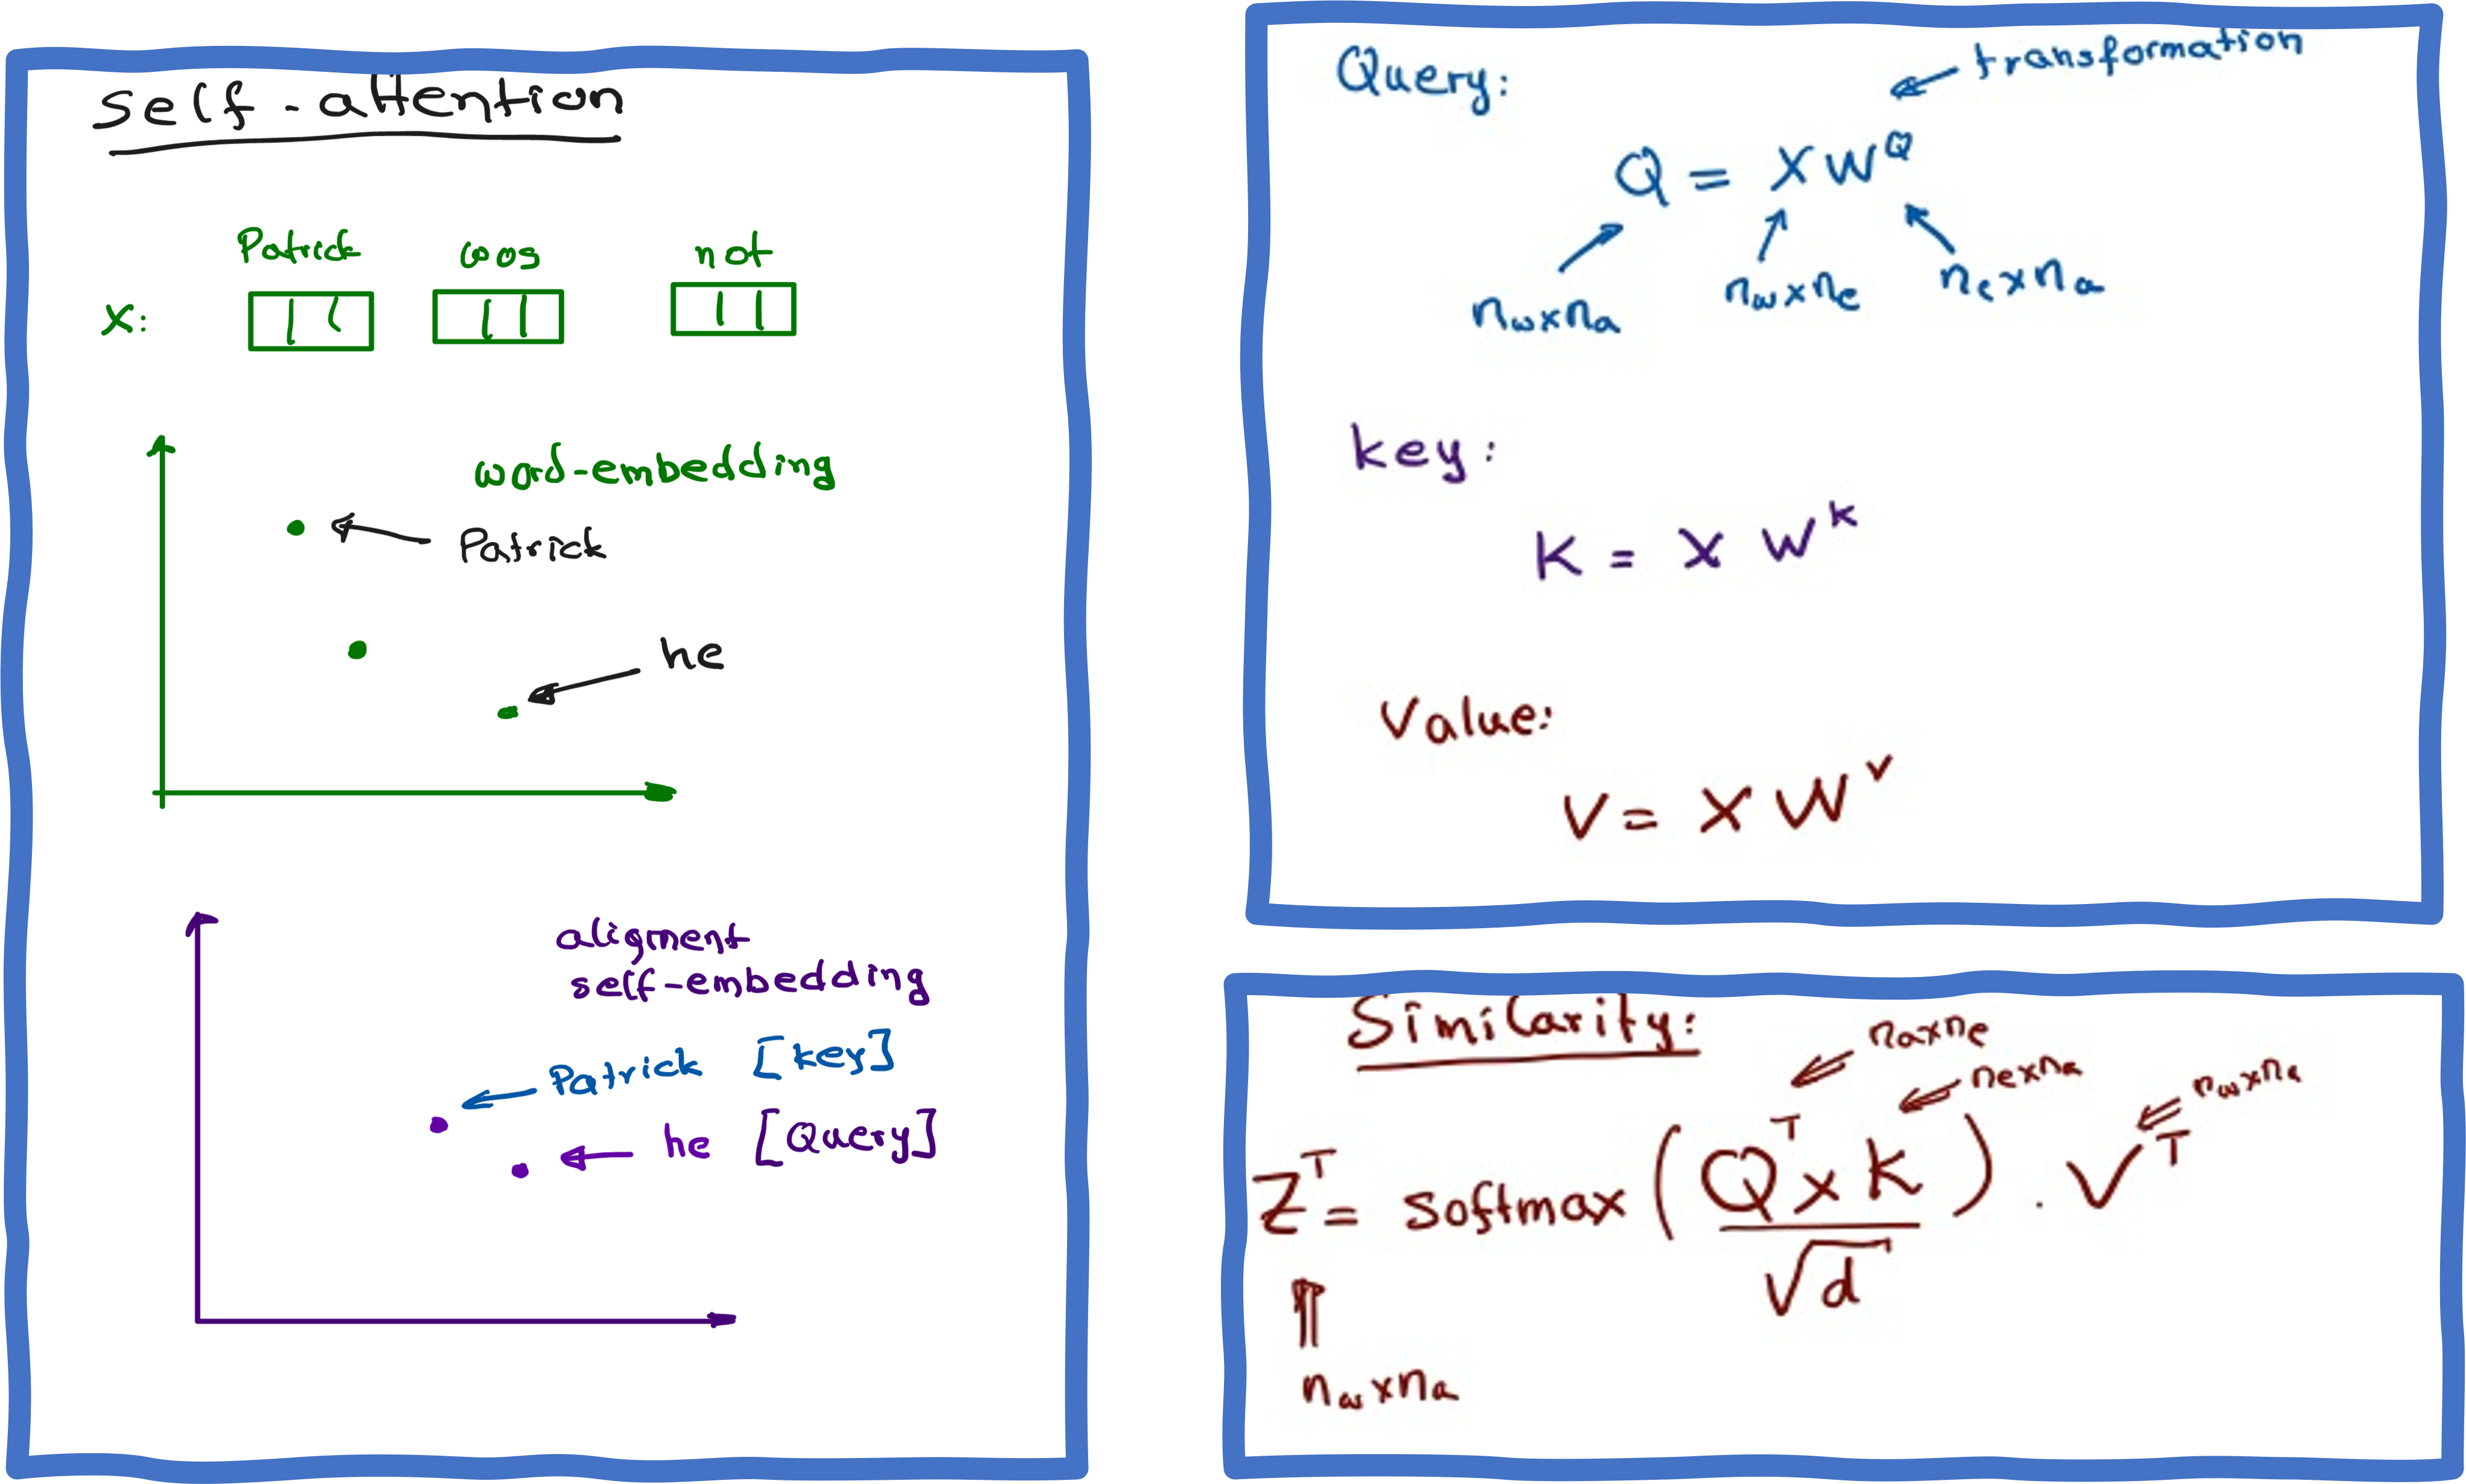
\includegraphics[width=\linewidth,keepaspectratio]{bert55}
	% \end{center}	
% \end{frame}

% %%%%%%%%%%%%%%%%%%%%%%%%%%%%%%%%%%%%%%%%%%%%%%%%%%%%%%%%%%%
% \begin{frame}[fragile]\frametitle{Transformers}

% \begin{columns}
    % \begin{column}[T]{0.5\linewidth}
			% \begin{center}
			% 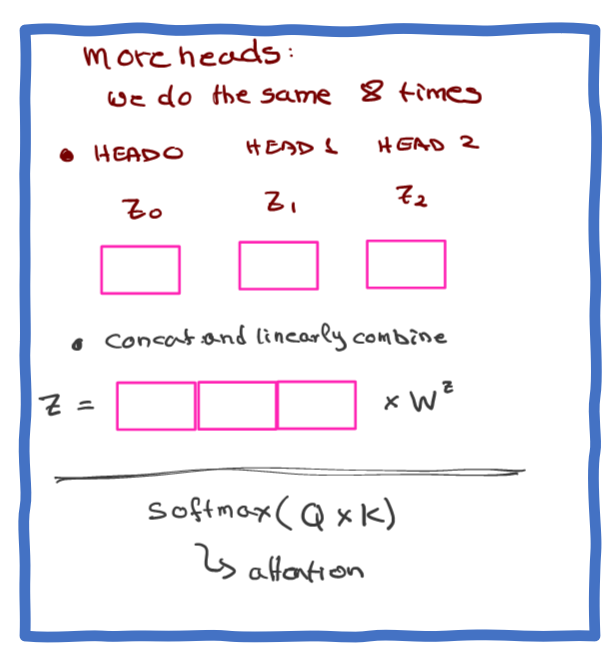
\includegraphics[width=\linewidth,keepaspectratio]{bert60}
			% \end{center}		
		% \end{column}
    % \begin{column}[T]{0.5\linewidth}
		% In the same fashion as CNN that we need more than one filter, transformers add a mechanism called ``multi-headed'' attention. This improves the performance of the attention layer in two ways:

      % \begin{itemize}
			% \item It expands the model's ability to focus on different positions.
			% \item It gives the attention layer multiple ``representation subspaces''
			% \end{itemize}
    % \end{column}
  % \end{columns}
			
% \end{frame}

% %%%%%%%%%%%%%%%%%%%%%%%%%%%%%%%%%%%%%%%%%%%%%%%%%%%%%%%%%%%
% \begin{frame}[fragile]\frametitle{Transformers}

% \begin{columns}
    % \begin{column}[T]{0.5\linewidth}
			% \begin{center}
			% 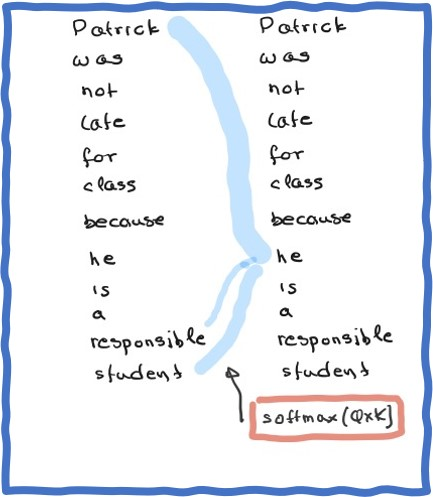
\includegraphics[width=\linewidth,keepaspectratio]{bert56}
			% \end{center}		
		% \end{column}
    % \begin{column}[T]{0.5\linewidth}
% As we encode the word ”he", one attention head is focusing most on ``Patrick'', while another is focusing on ``student'' -- in a sense, the model's representation of the word ``he'' combines the representations of both ``Patrick'' and ``stduent''.

    % \end{column}
  % \end{columns}
			
% \end{frame}

% %%%%%%%%%%%%%%%%%%%%%%%%%%%%%%%%%%%%%%%%%%%%%%%%%%%%%%%%%%%
% \begin{frame}[fragile]\frametitle{Transformers}


			% \begin{center}
			% 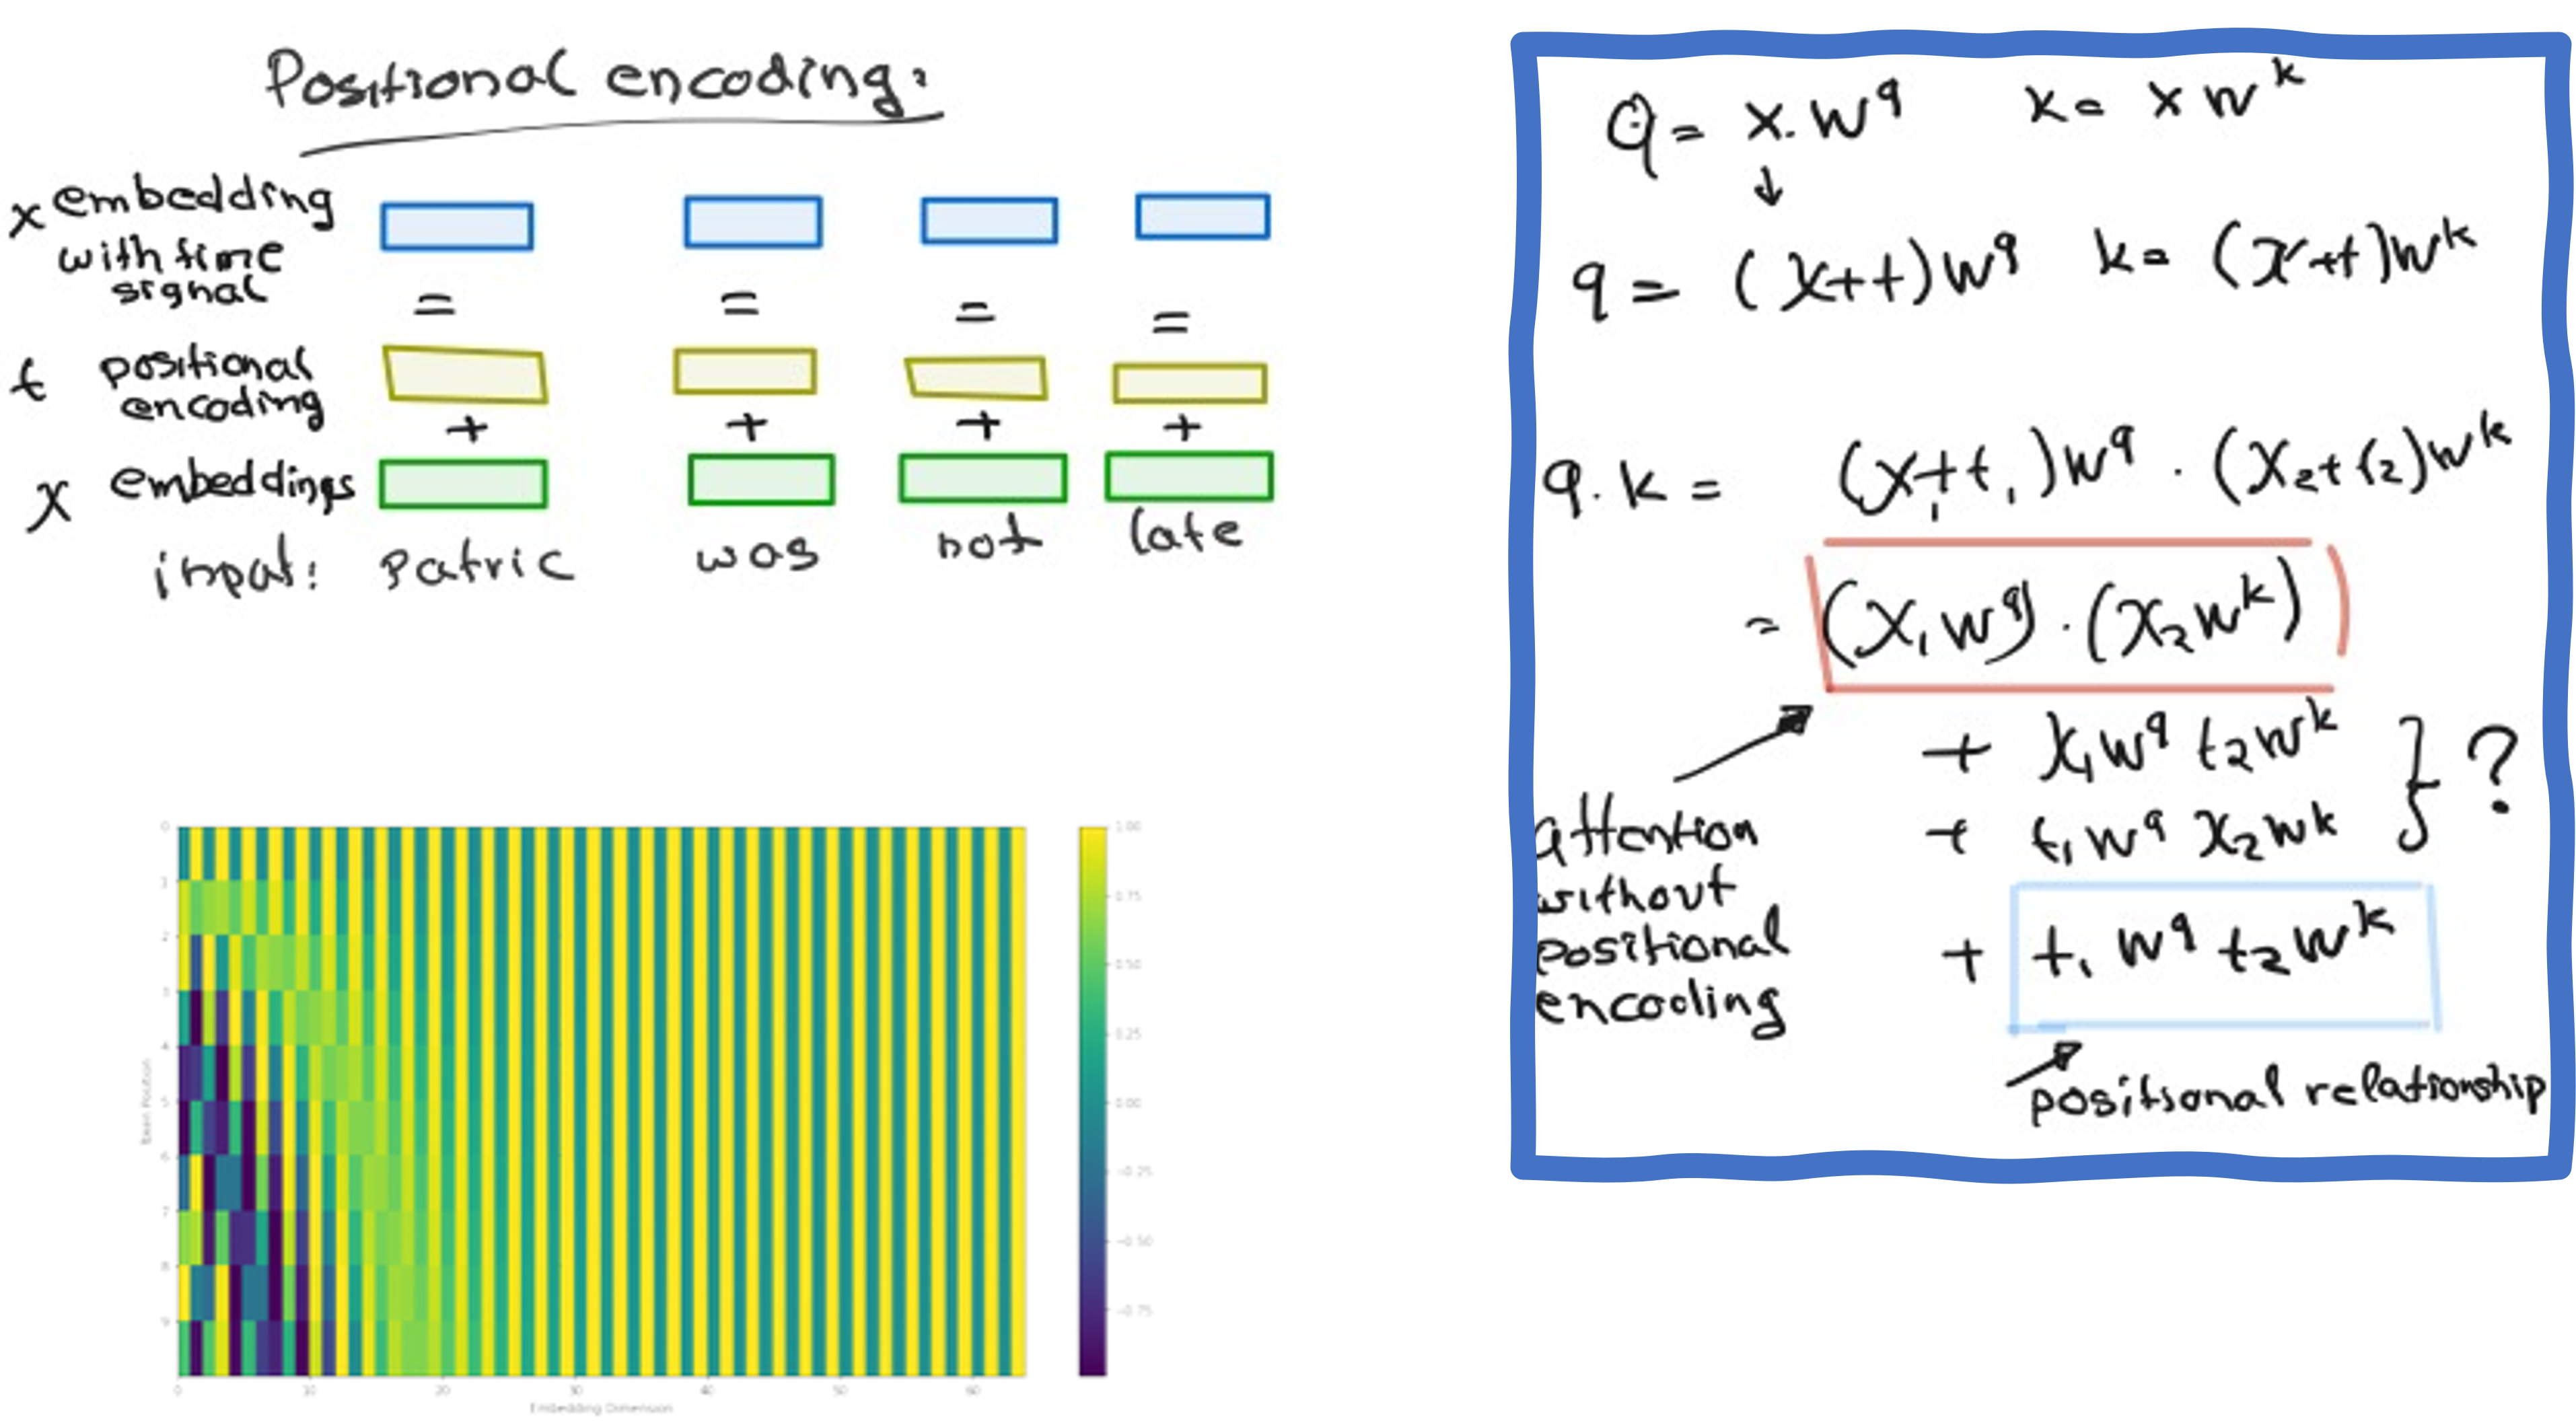
\includegraphics[width=\linewidth,keepaspectratio]{bert57}
			% \end{center}		

			
% \end{frame}


% %%%%%%%%%%%%%%%%%%%%%%%%%%%%%%%%%%%%%%%%%%%%%%%%%%%%%%%%%%%
% \begin{frame}[fragile]\frametitle{Transformers}

% \begin{columns}
    % \begin{column}[T]{0.5\linewidth}
			% \begin{center}
			% 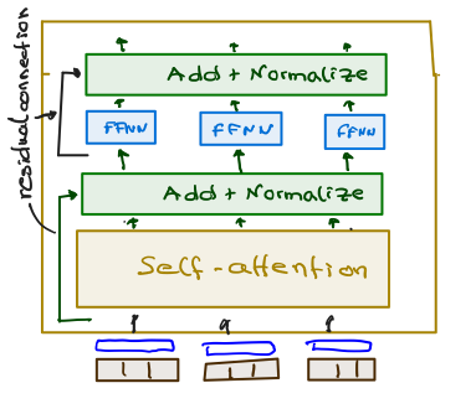
\includegraphics[width=\linewidth,keepaspectratio]{bert61}
			% \end{center}		
		% \end{column}
    % \begin{column}[T]{0.5\linewidth}
      % \begin{itemize}
			% \item Details in the architecture of the encoder:
			% \item Each sub-layer  in each encoder has a residual connection around it
			% \item And a layer-normalization step.
			% \end{itemize}
    % \end{column}
  % \end{columns}
			
% \end{frame}

% %%%%%%%%%%%%%%%%%%%%%%%%%%%%%%%%%%%%%%%%%%%%%%%%%%%%%%%%%%%
% \begin{frame}[fragile]\frametitle{Transformers}


			% \begin{center}
			% 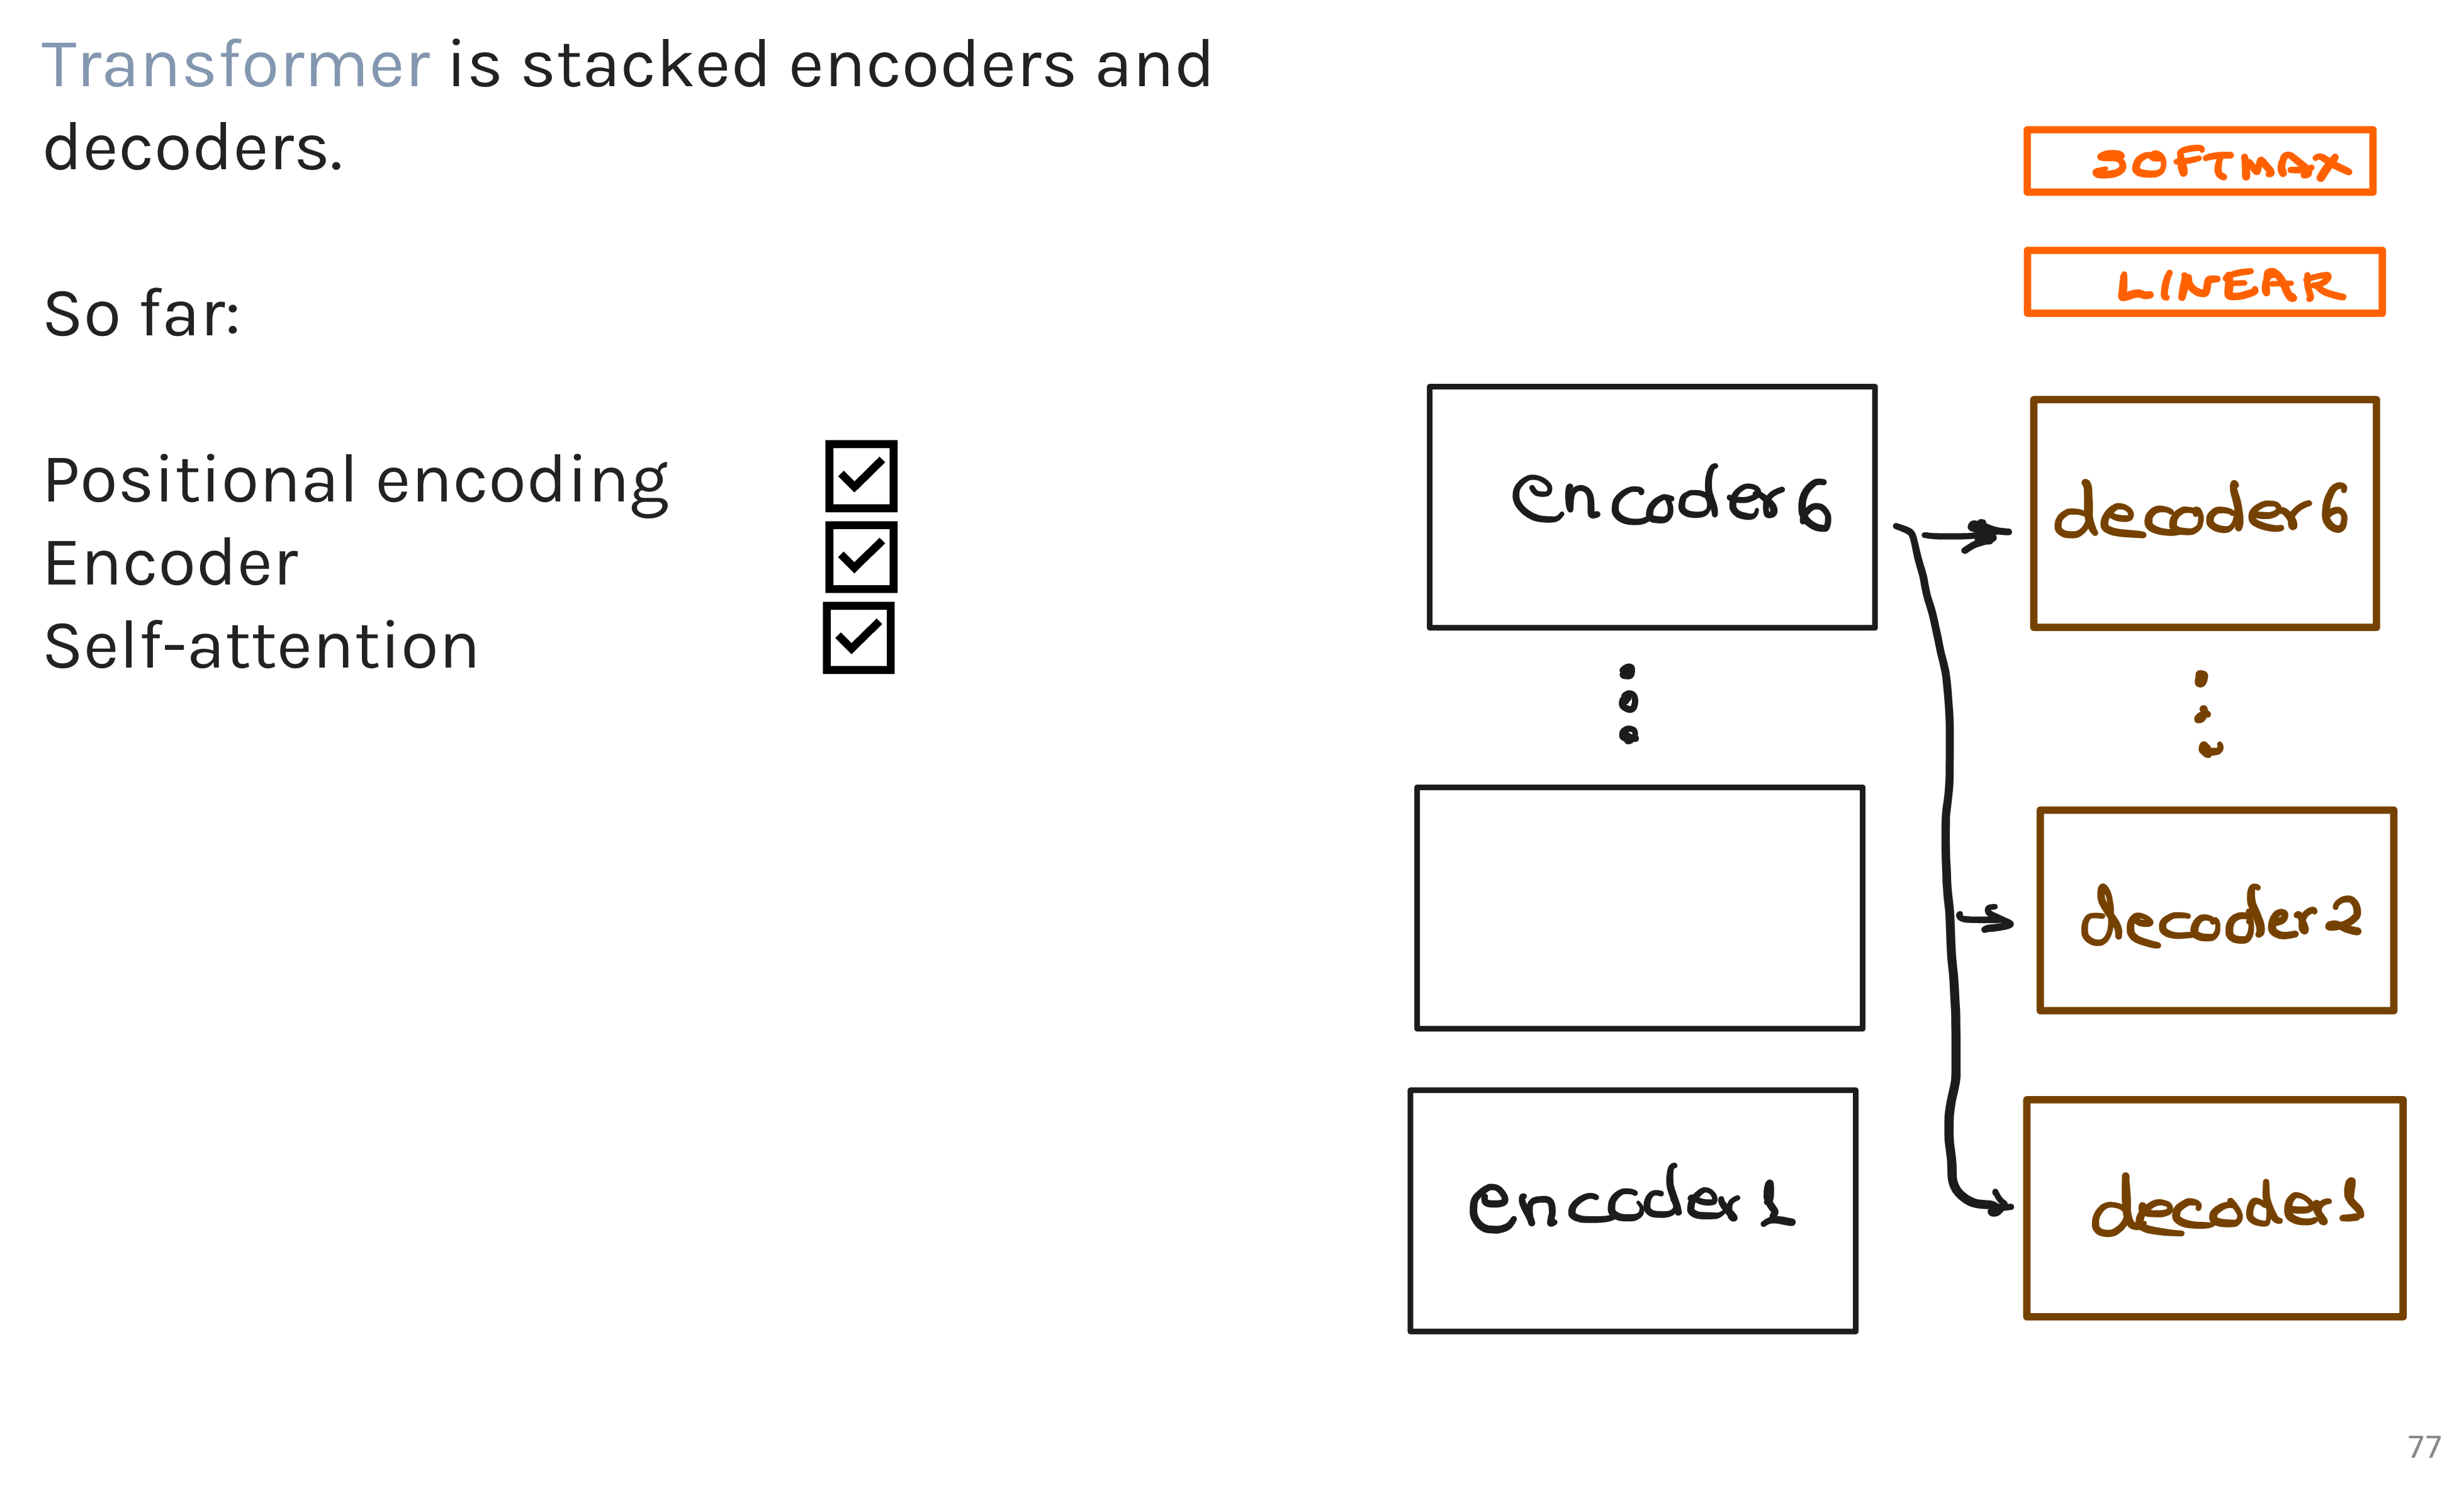
\includegraphics[width=\linewidth,keepaspectratio]{bert62}
			% \end{center}		

			
% \end{frame}

% %%%%%%%%%%%%%%%%%%%%%%%%%%%%%%%%%%%%%%%%%%%%%%%%%%%%%%%%%%%
% \begin{frame}[fragile]\frametitle{Transformers}


			% \begin{center}
			% 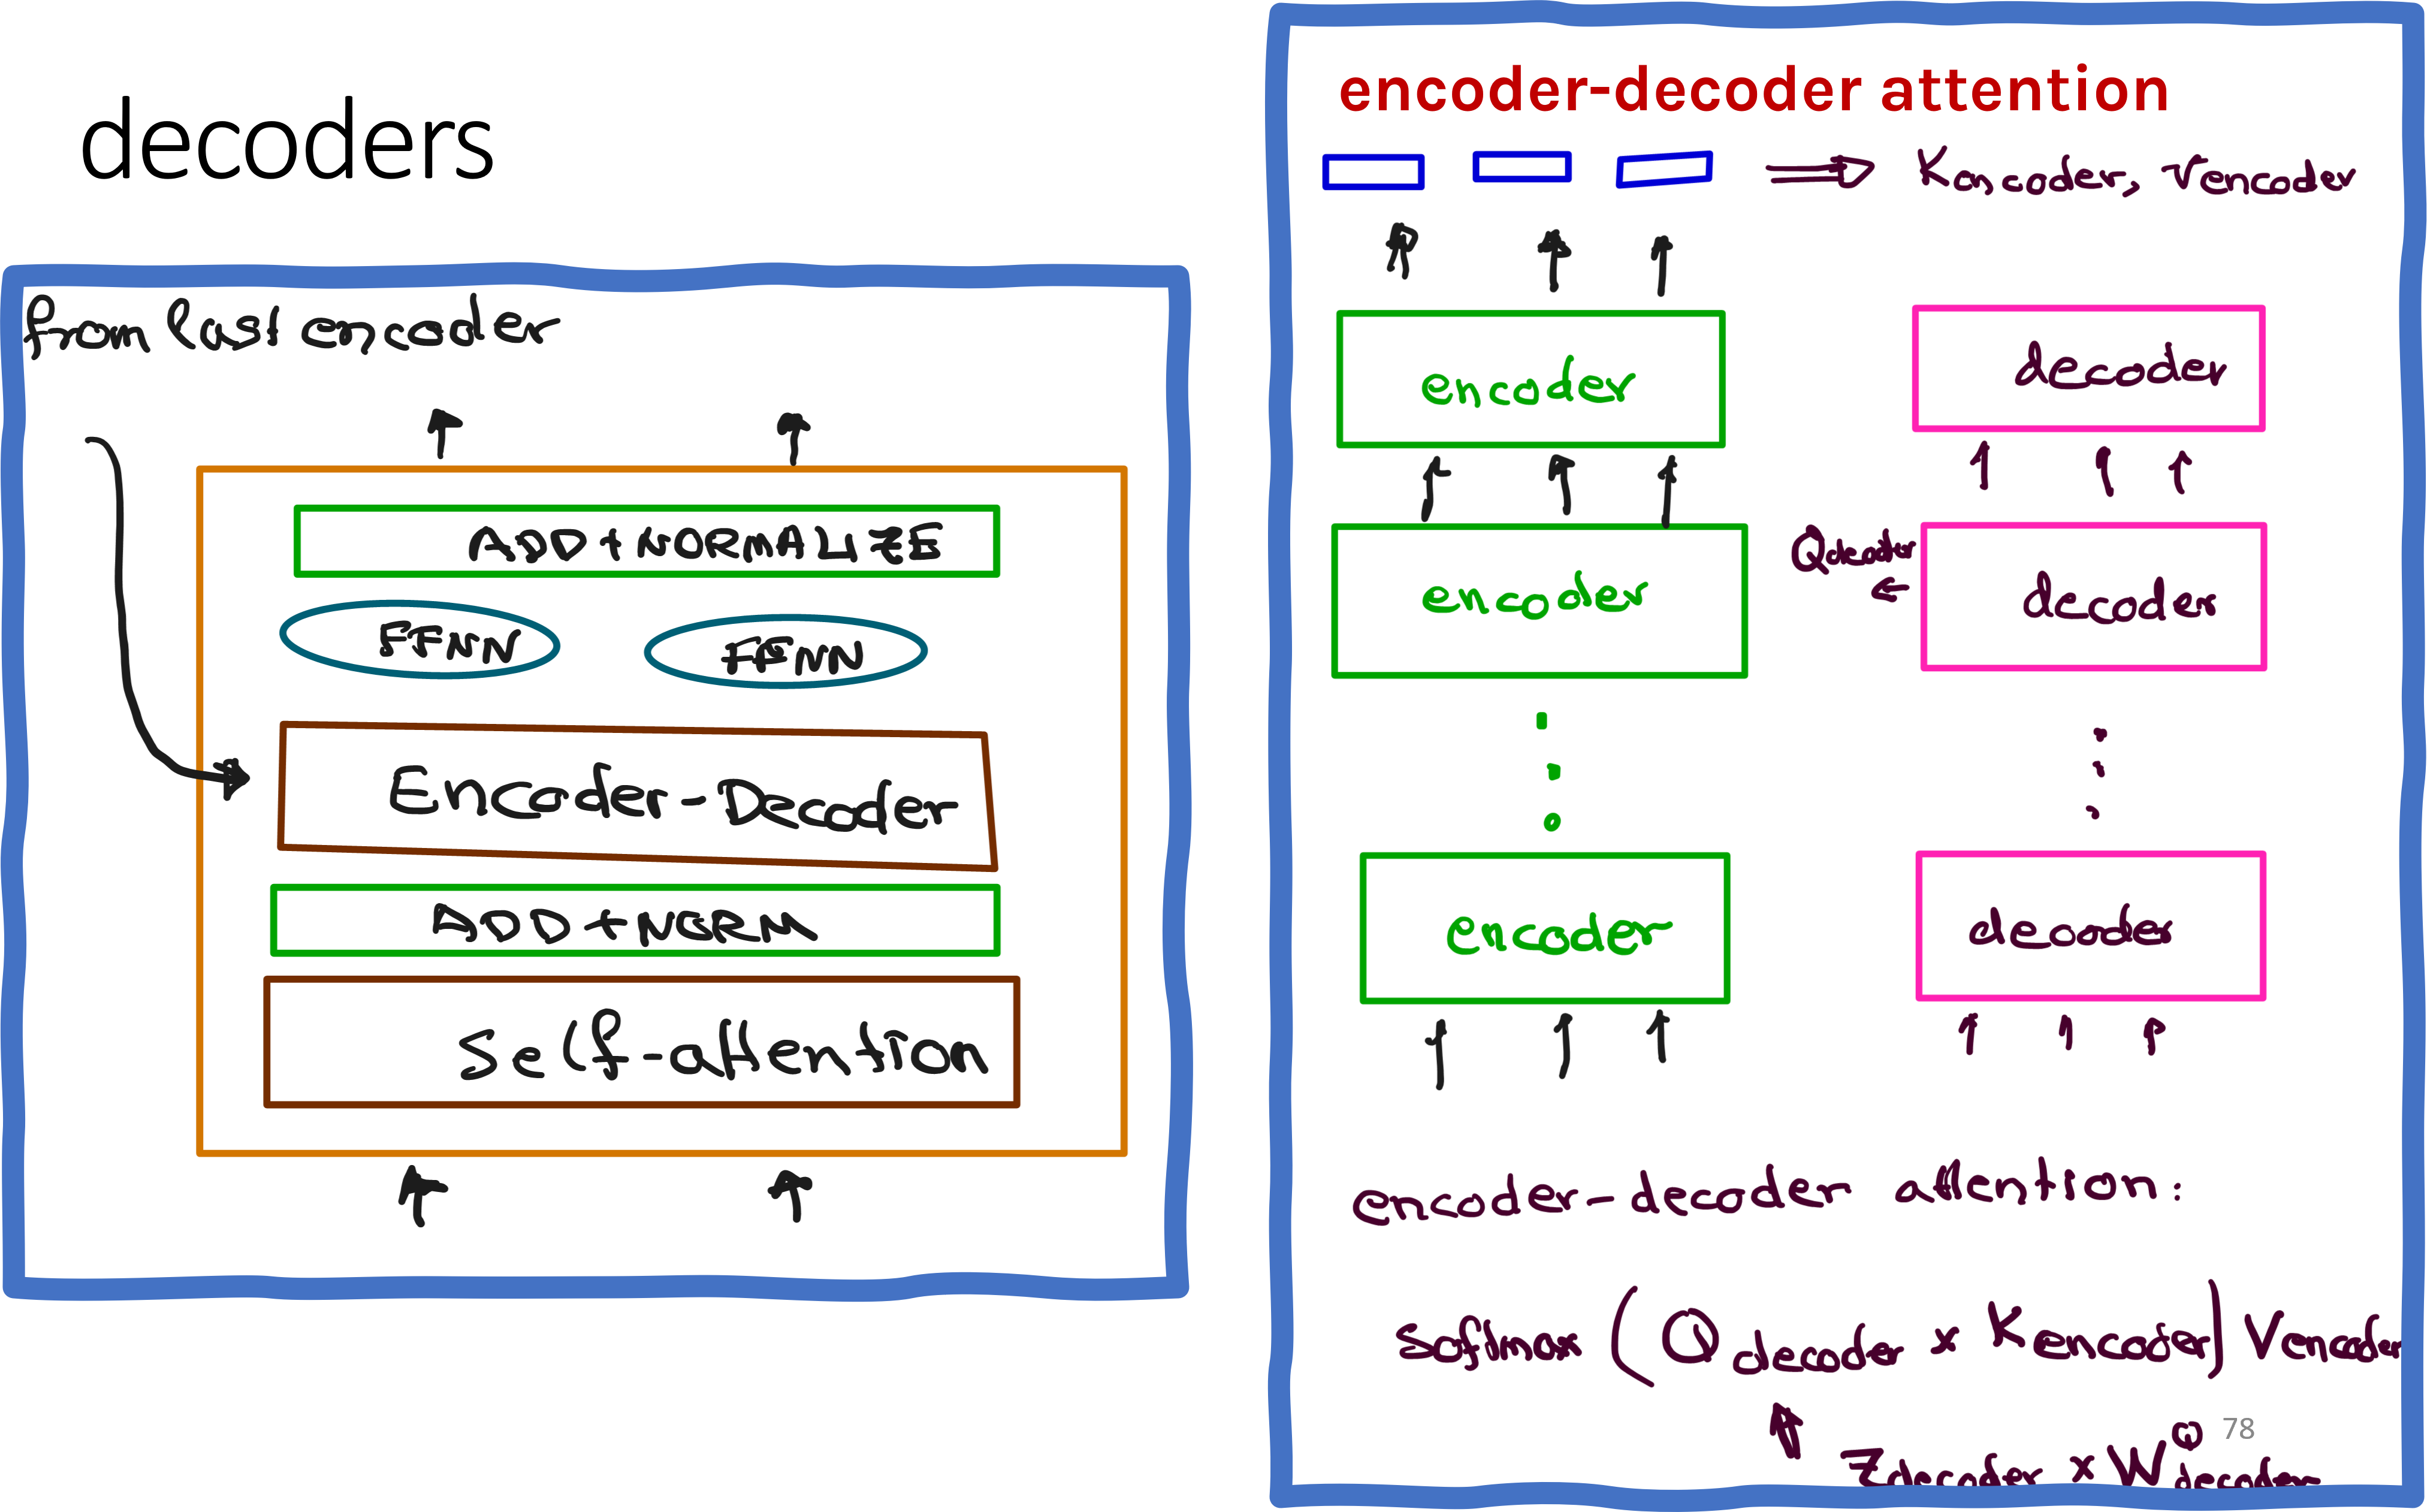
\includegraphics[width=\linewidth,keepaspectratio]{bert63}
			% \end{center}		

			
% \end{frame}

% %%%%%%%%%%%%%%%%%%%%%%%%%%%%%%%%%%%%%%%%%%%%%%%%%%%%%%%%%%%
% \begin{frame}[fragile]\frametitle{The Final Linear and Softmax Layer}


			% \begin{center}
			% 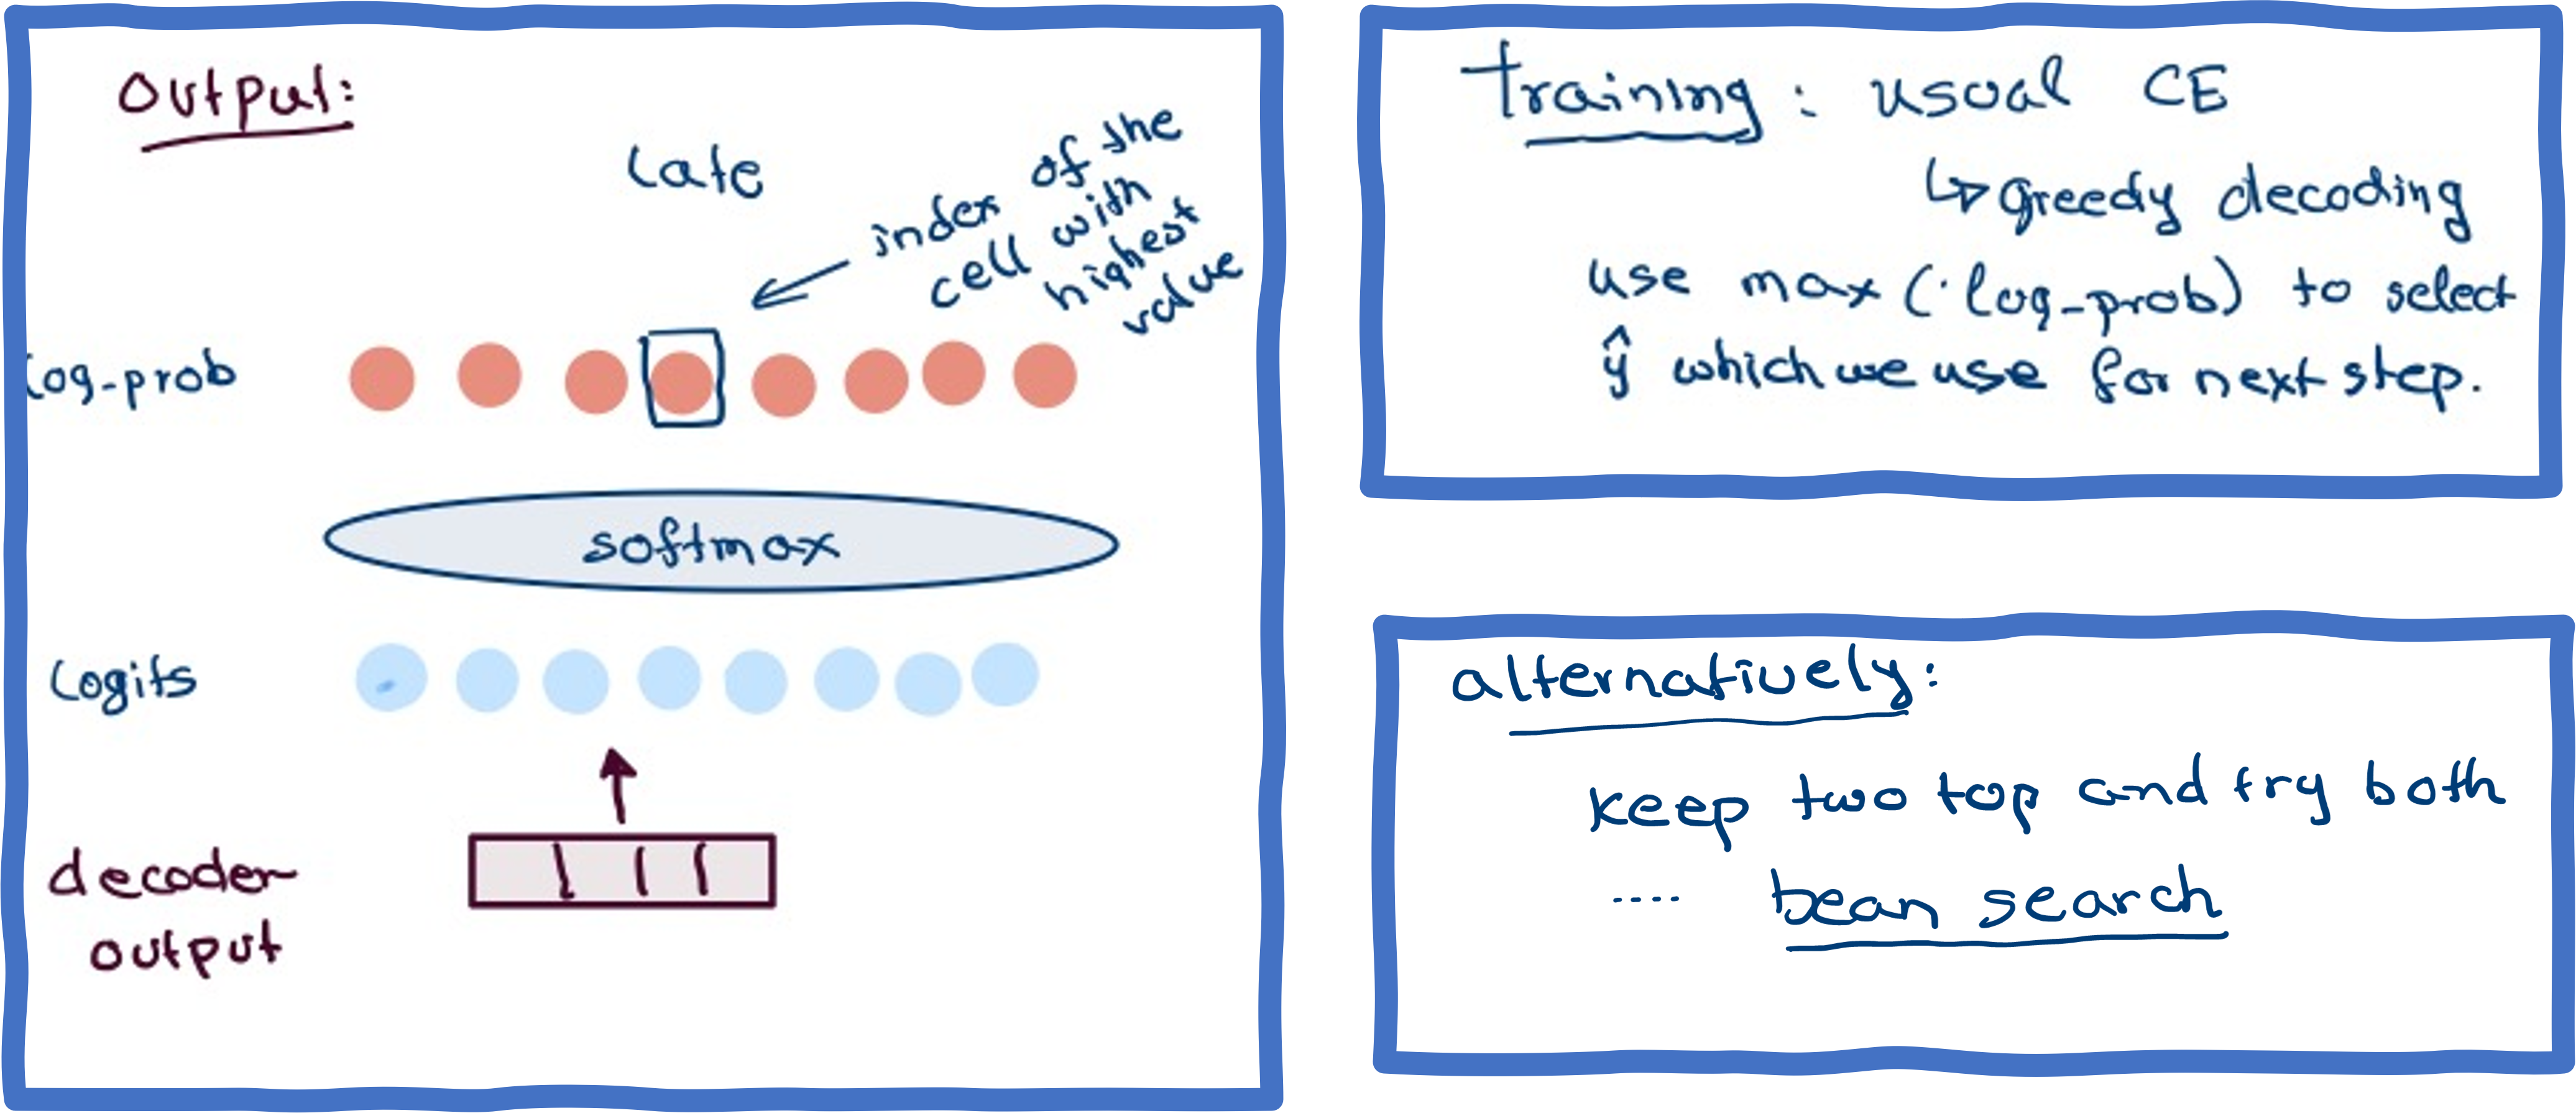
\includegraphics[width=\linewidth,keepaspectratio]{bert64}
			% \end{center}		

			
% \end{frame}

%%%%%%%%%%%%%%%%%%%%%%%%%%%%%%%%%%%%%%%%%%%%%%%%%%%%%%%%%%%
\begin{frame}[fragile]\frametitle{Conclusion}

Main innovations in Transformers:
\begin{itemize}
\item Positional Encoding: instead of architecture relying on sequence order, like RNNs, the Transformers store the position, making them order independent architecturally as the position is part of th data itself so that you can then have parallel processing
\item Self-attention: Weights vector, how much each word contributes, learnt by seeing many pairs, during training. Self, meaning within itself. Internal structure understanding, Encoder only.

			\end{itemize}
			
\end{frame}


% %%%%%%%%%%%%%%%%%%%%%%%%%%%%%%%%%%%%%%%%%%%%%%%%%%%%%%%%%%%
% \begin{frame}[fragile]\frametitle{Results}
% Great Results with Transformers
			
			% \begin{center}
			% 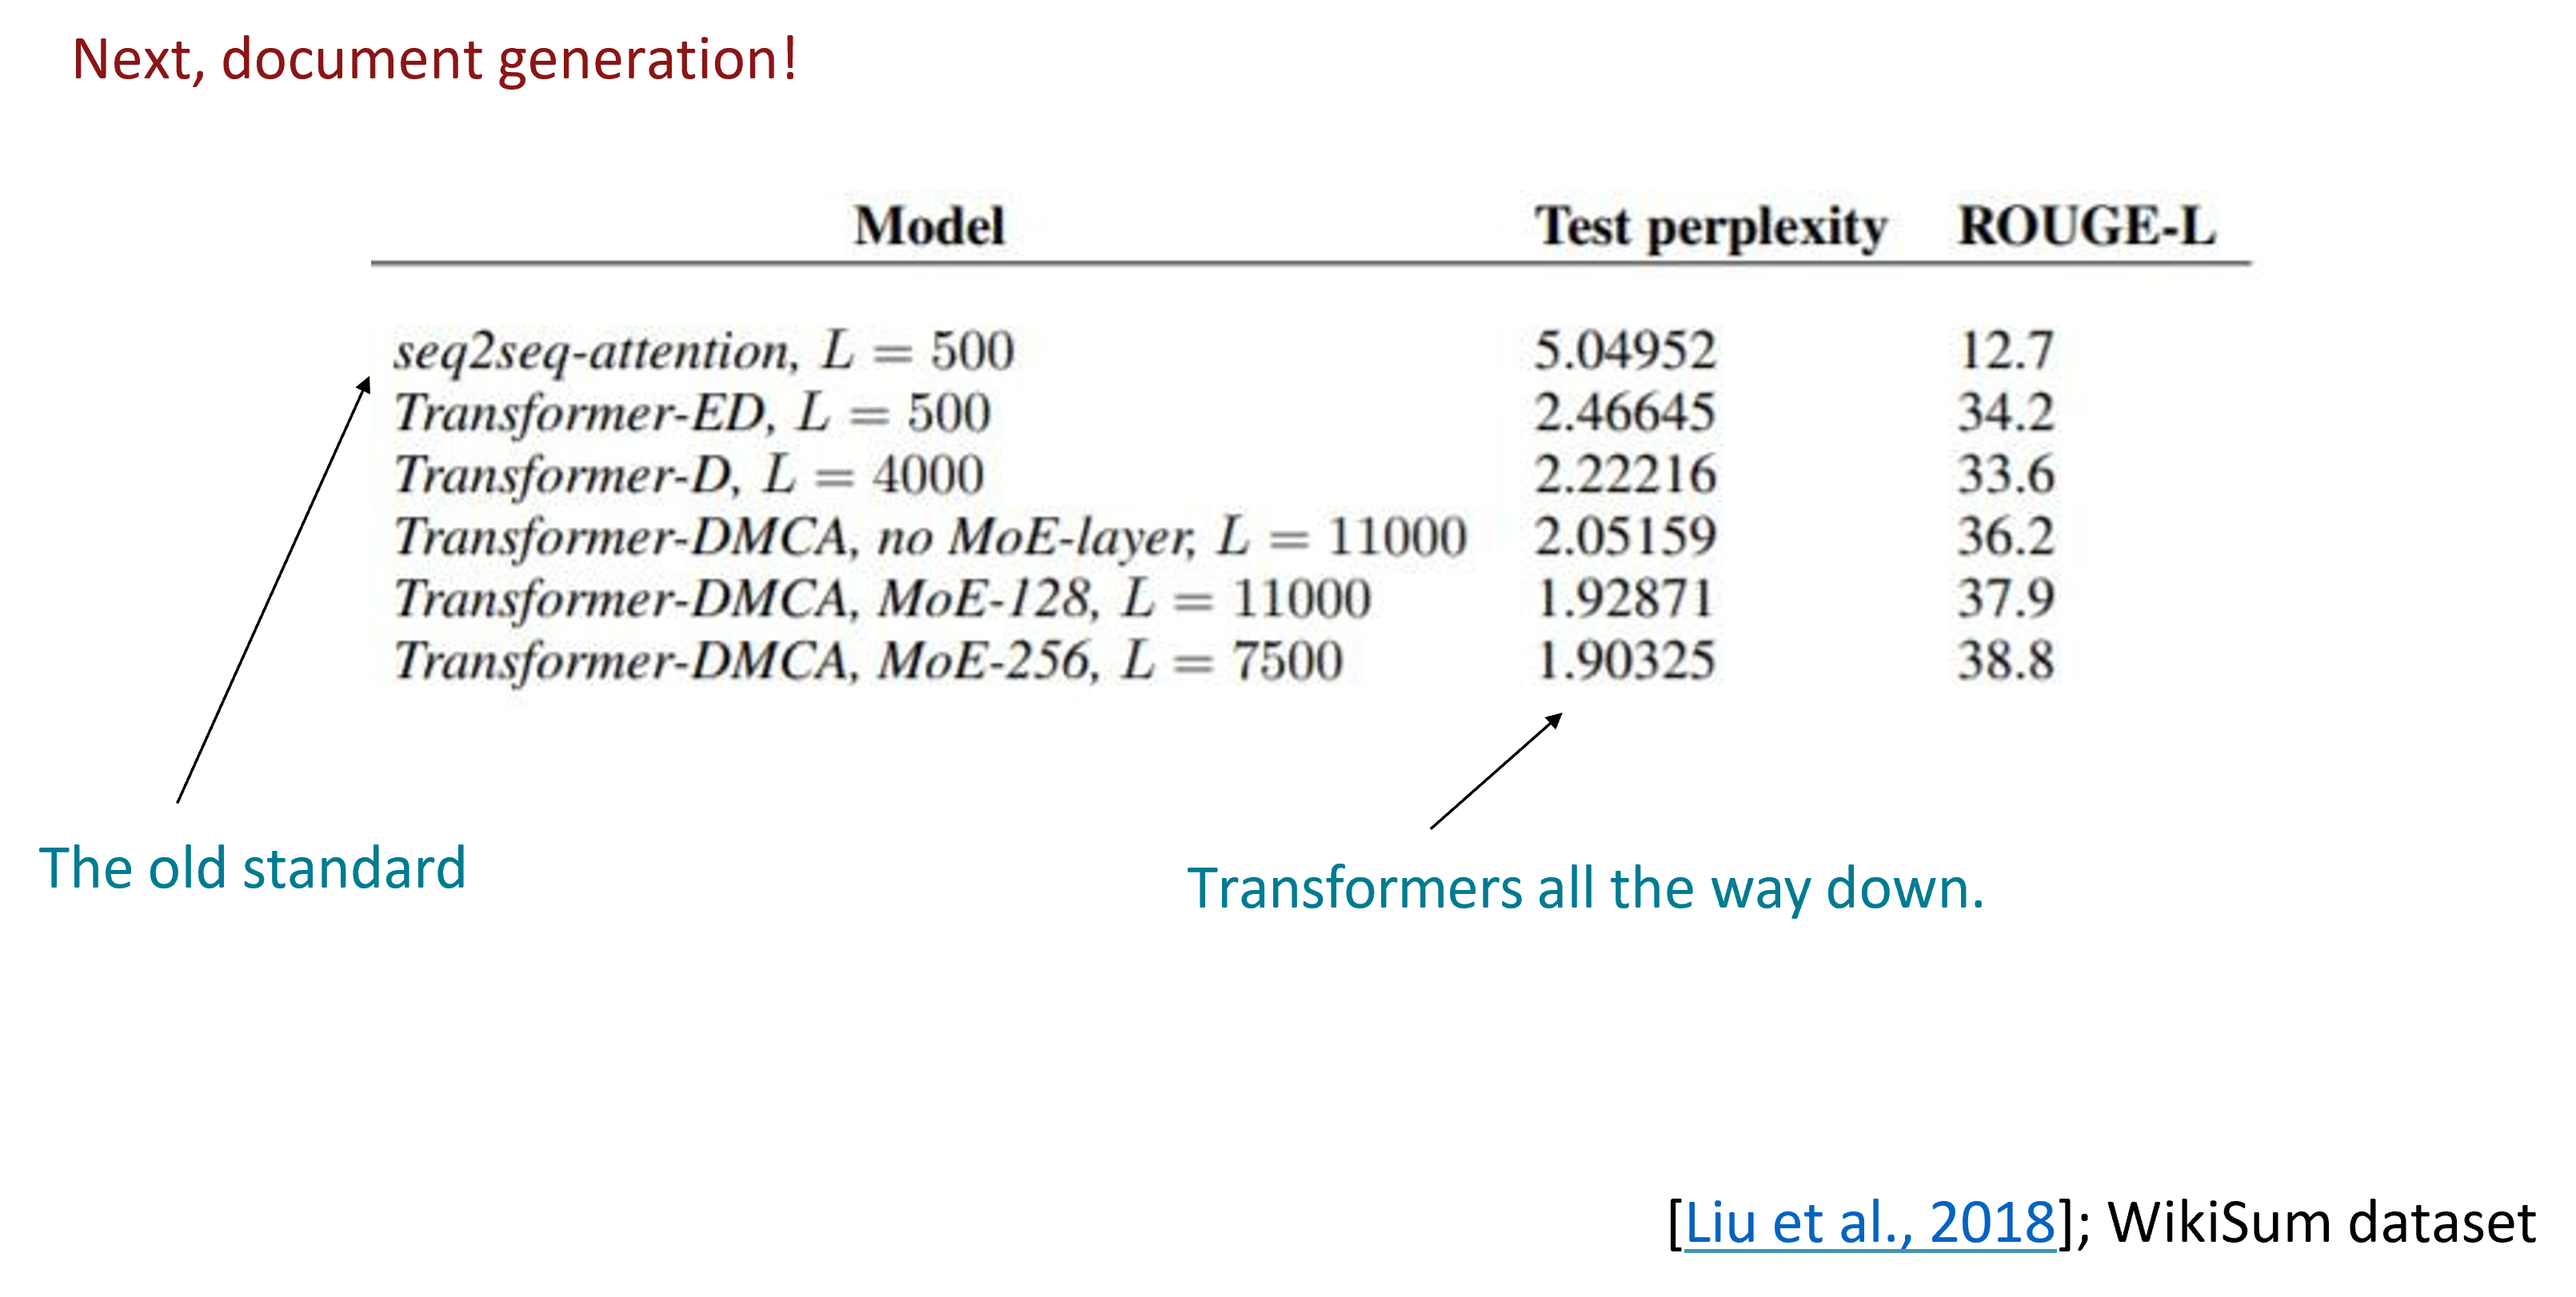
\includegraphics[width=\linewidth,keepaspectratio]{bert91}
			% \end{center}		
			
			% % {\tiny (Ref: John Hewitt)}

% \end{frame}

% %%%%%%%%%%%%%%%%%%%%%%%%%%%%%%%%%%%%%%%%%%%%%%%%%%%%%%%%%%%
% \begin{frame}[fragile]\frametitle{Issues}

% What would we like to fix about the Transformer?

      % \begin{itemize}
			% \item Quadratic compute in self-attention:
			      % \begin{itemize}
						% \item Computing all pairs of interactions means our computation grows quadratically with the sequence length!
						% \item For recurrent models, it only grew linearly!
						% \end{itemize}
			% \item Position representations:
			      % \begin{itemize}
						% \item Are simple absolute indices the best we can do to represent position?
						% \item Relative linear position attention [Shaw et al., 2018]
						% \item Dependency syntax-based position [Wang et al., 2019]			
						% \end{itemize}
			% \end{itemize}

			% % {\tiny (Ref: John Hewitt)}

% \end{frame}

% %%%%%%%%%%%%%%%%%%%%%%%%%%%%%%%%%%%%%%%%%%%%%%%%%%%%%%%%%%%
% \begin{frame}[fragile]\frametitle{Quadratic computation as function of seq. length}

			
			% \begin{center}
			% 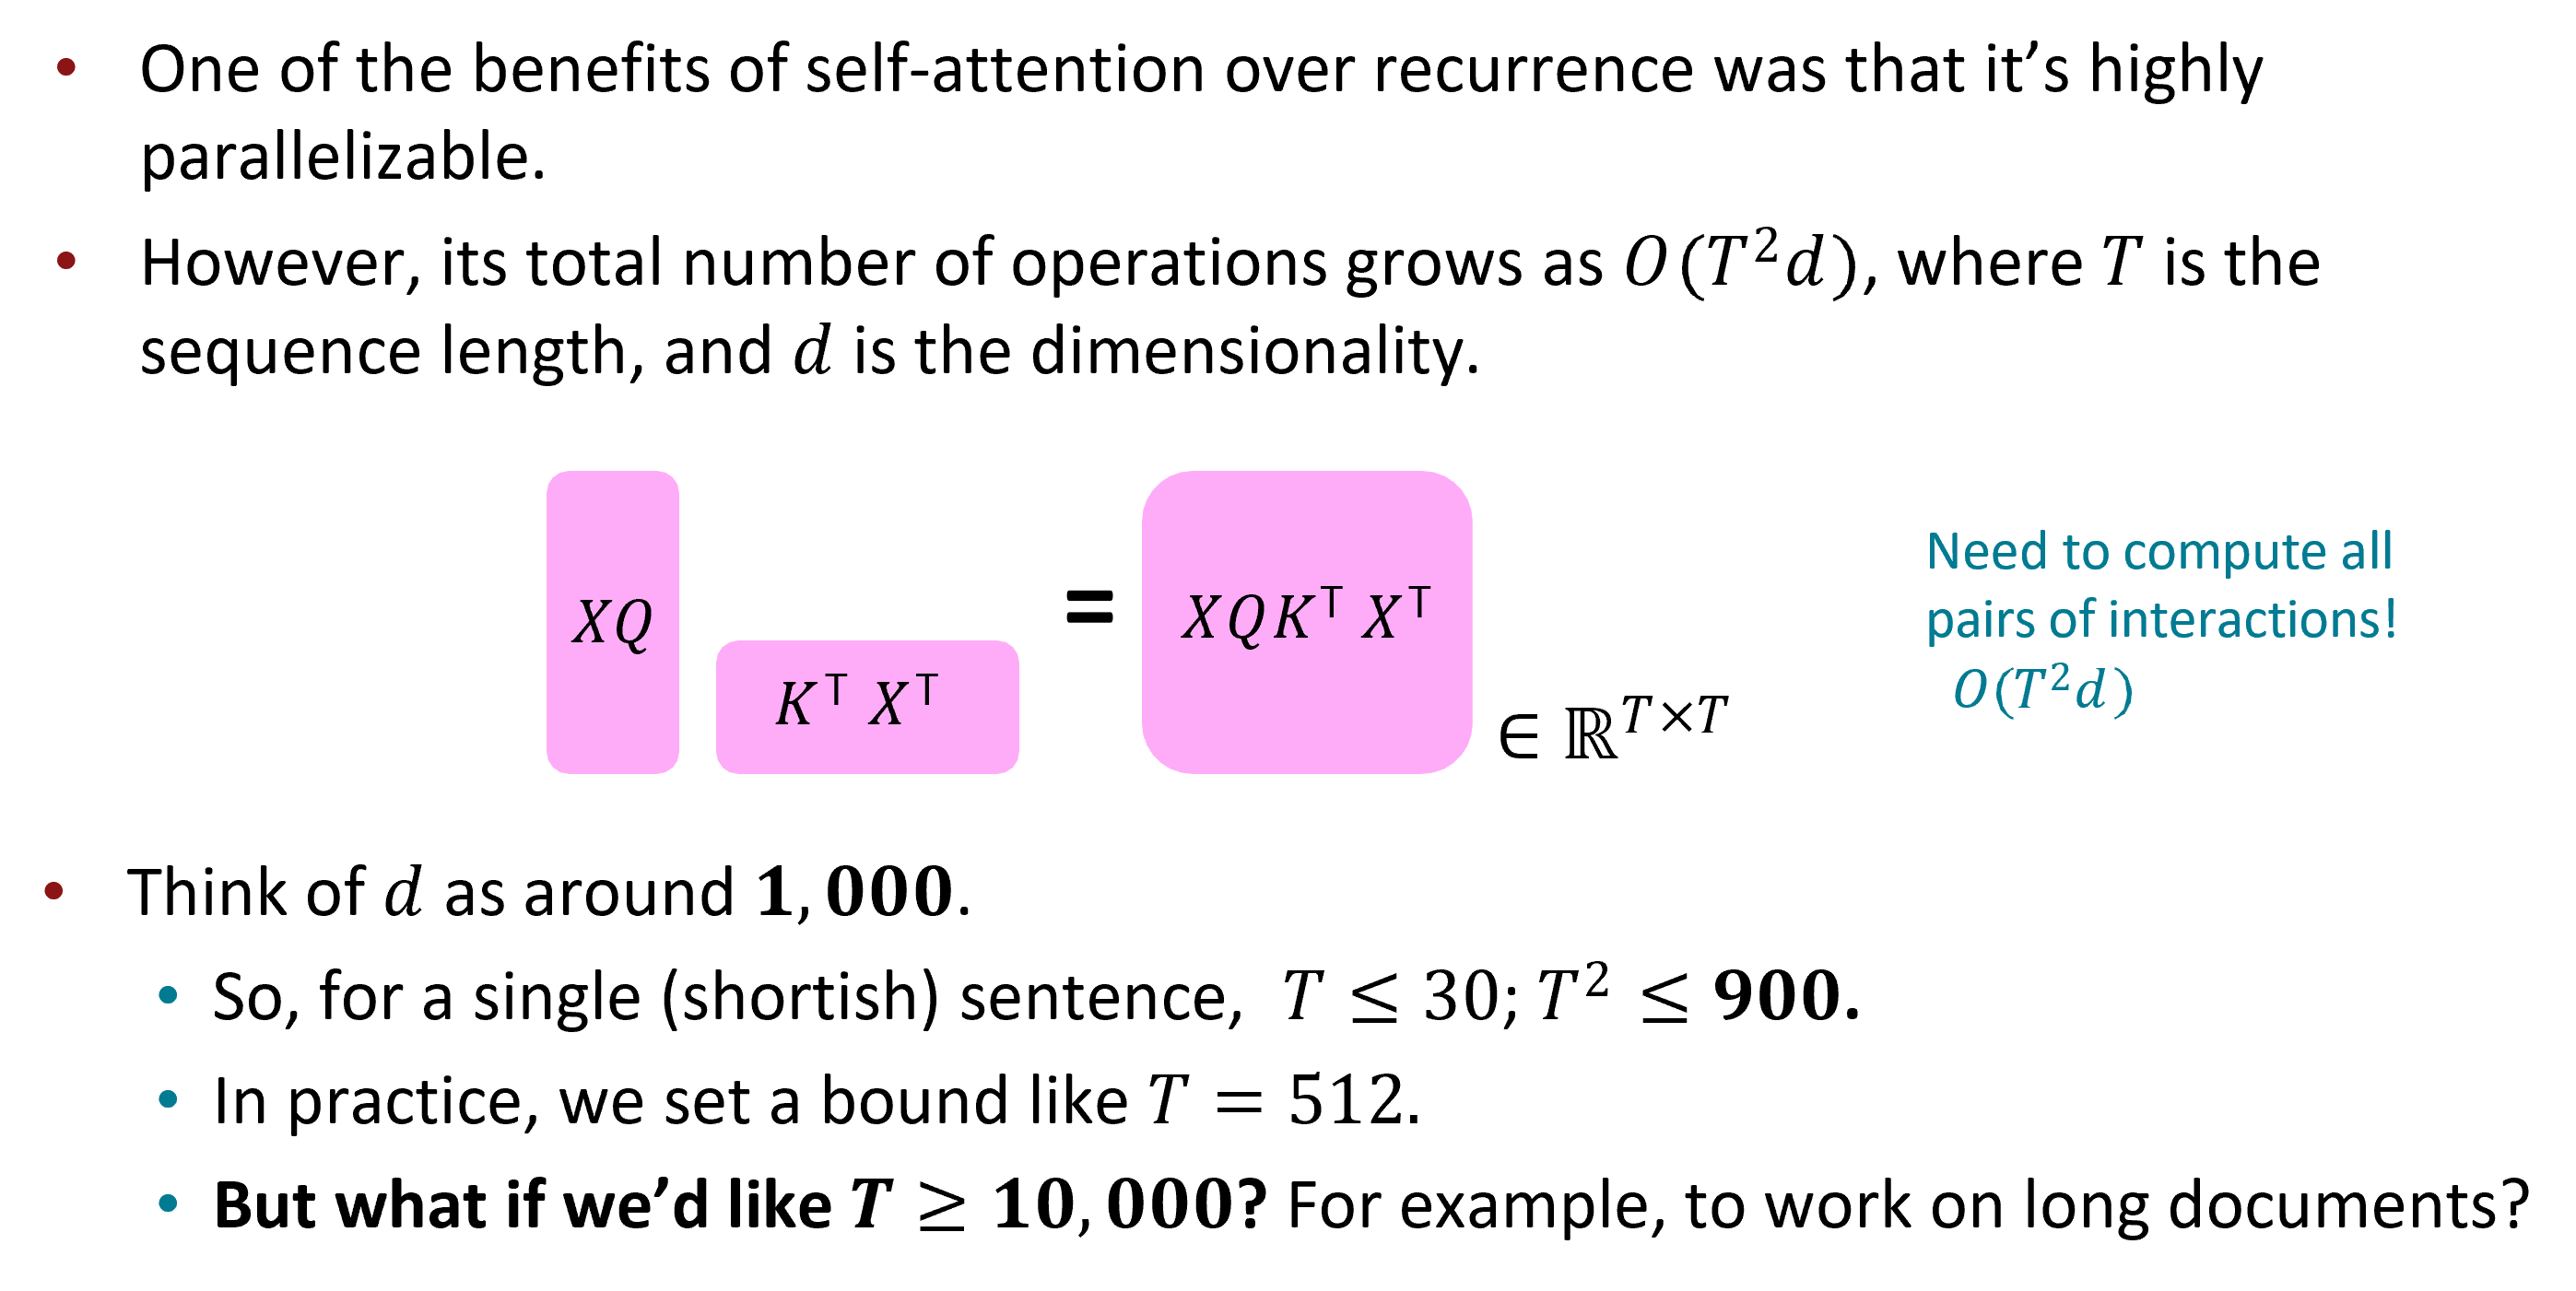
\includegraphics[width=\linewidth,keepaspectratio]{bert92}
			% \end{center}		
			
			% % {\tiny (Ref: John Hewitt)}

% \end{frame}

% %%%%%%%%%%%%%%%%%%%%%%%%%%%%%%%%%%%%%%%%%%%%%%%%%%%%%%%%%%%
% \begin{frame}[fragile]\frametitle{Recent work on improving on quadratic self-attention cost}

			
			% \begin{center}
			% 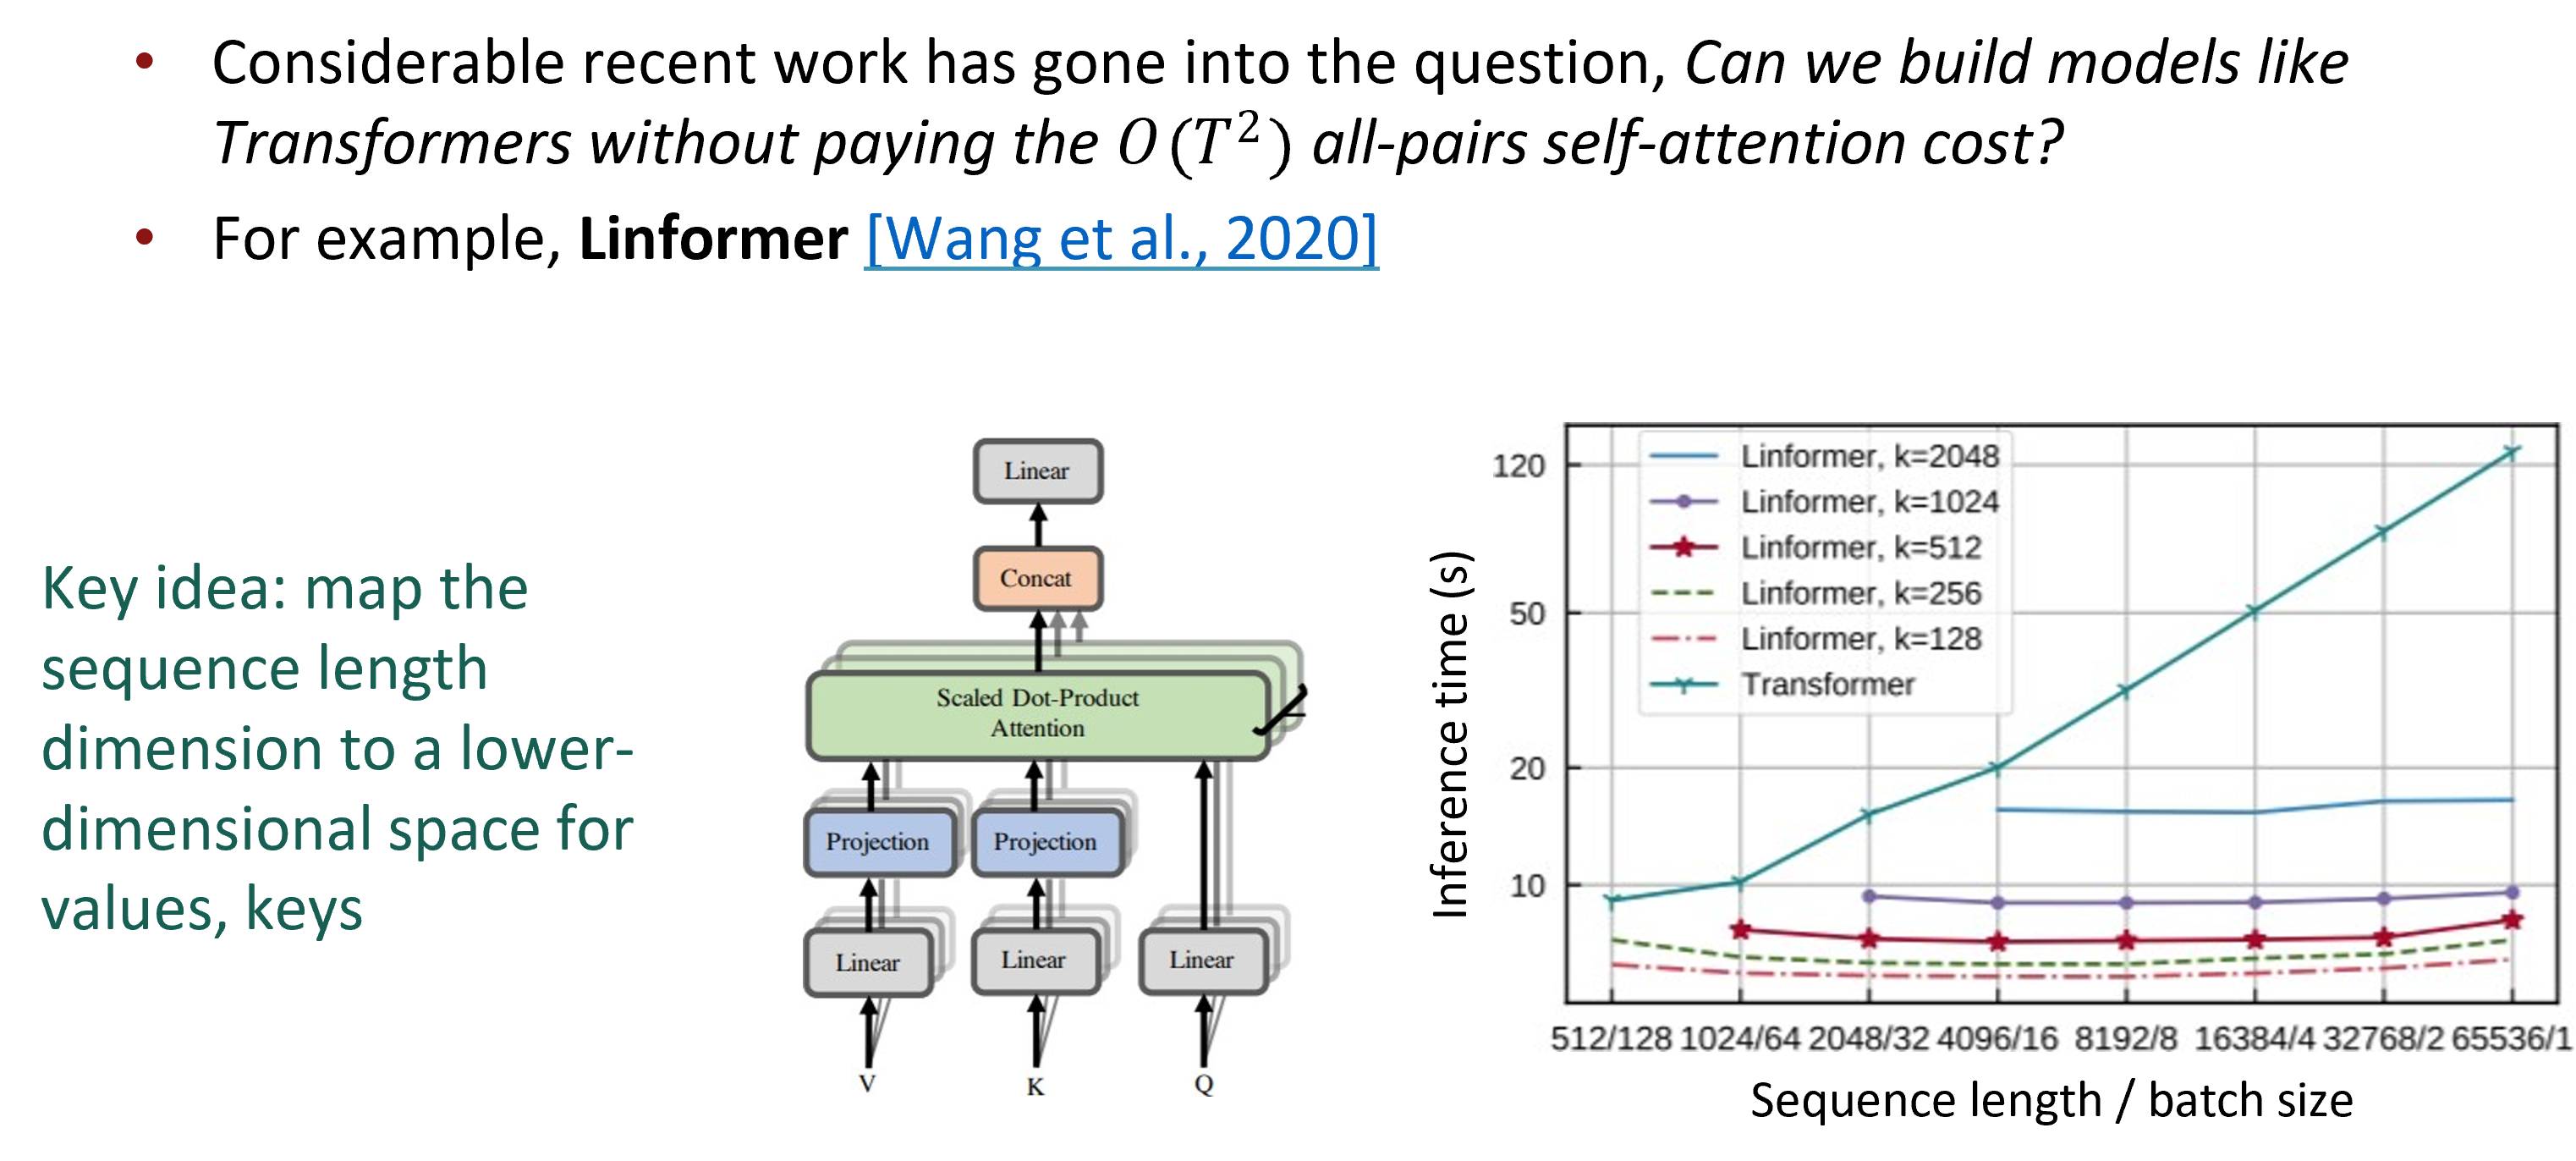
\includegraphics[width=\linewidth,keepaspectratio]{bert93}
			% \end{center}		
			
			% % {\tiny (Ref: John Hewitt)}

% \end{frame}

% %%%%%%%%%%%%%%%%%%%%%%%%%%%%%%%%%%%%%%%%%%%%%%%%%%%%%%%%%%%
% \begin{frame}[fragile]\frametitle{Recent work on improving on quadratic self-attention cost}

			
			% \begin{center}
			% 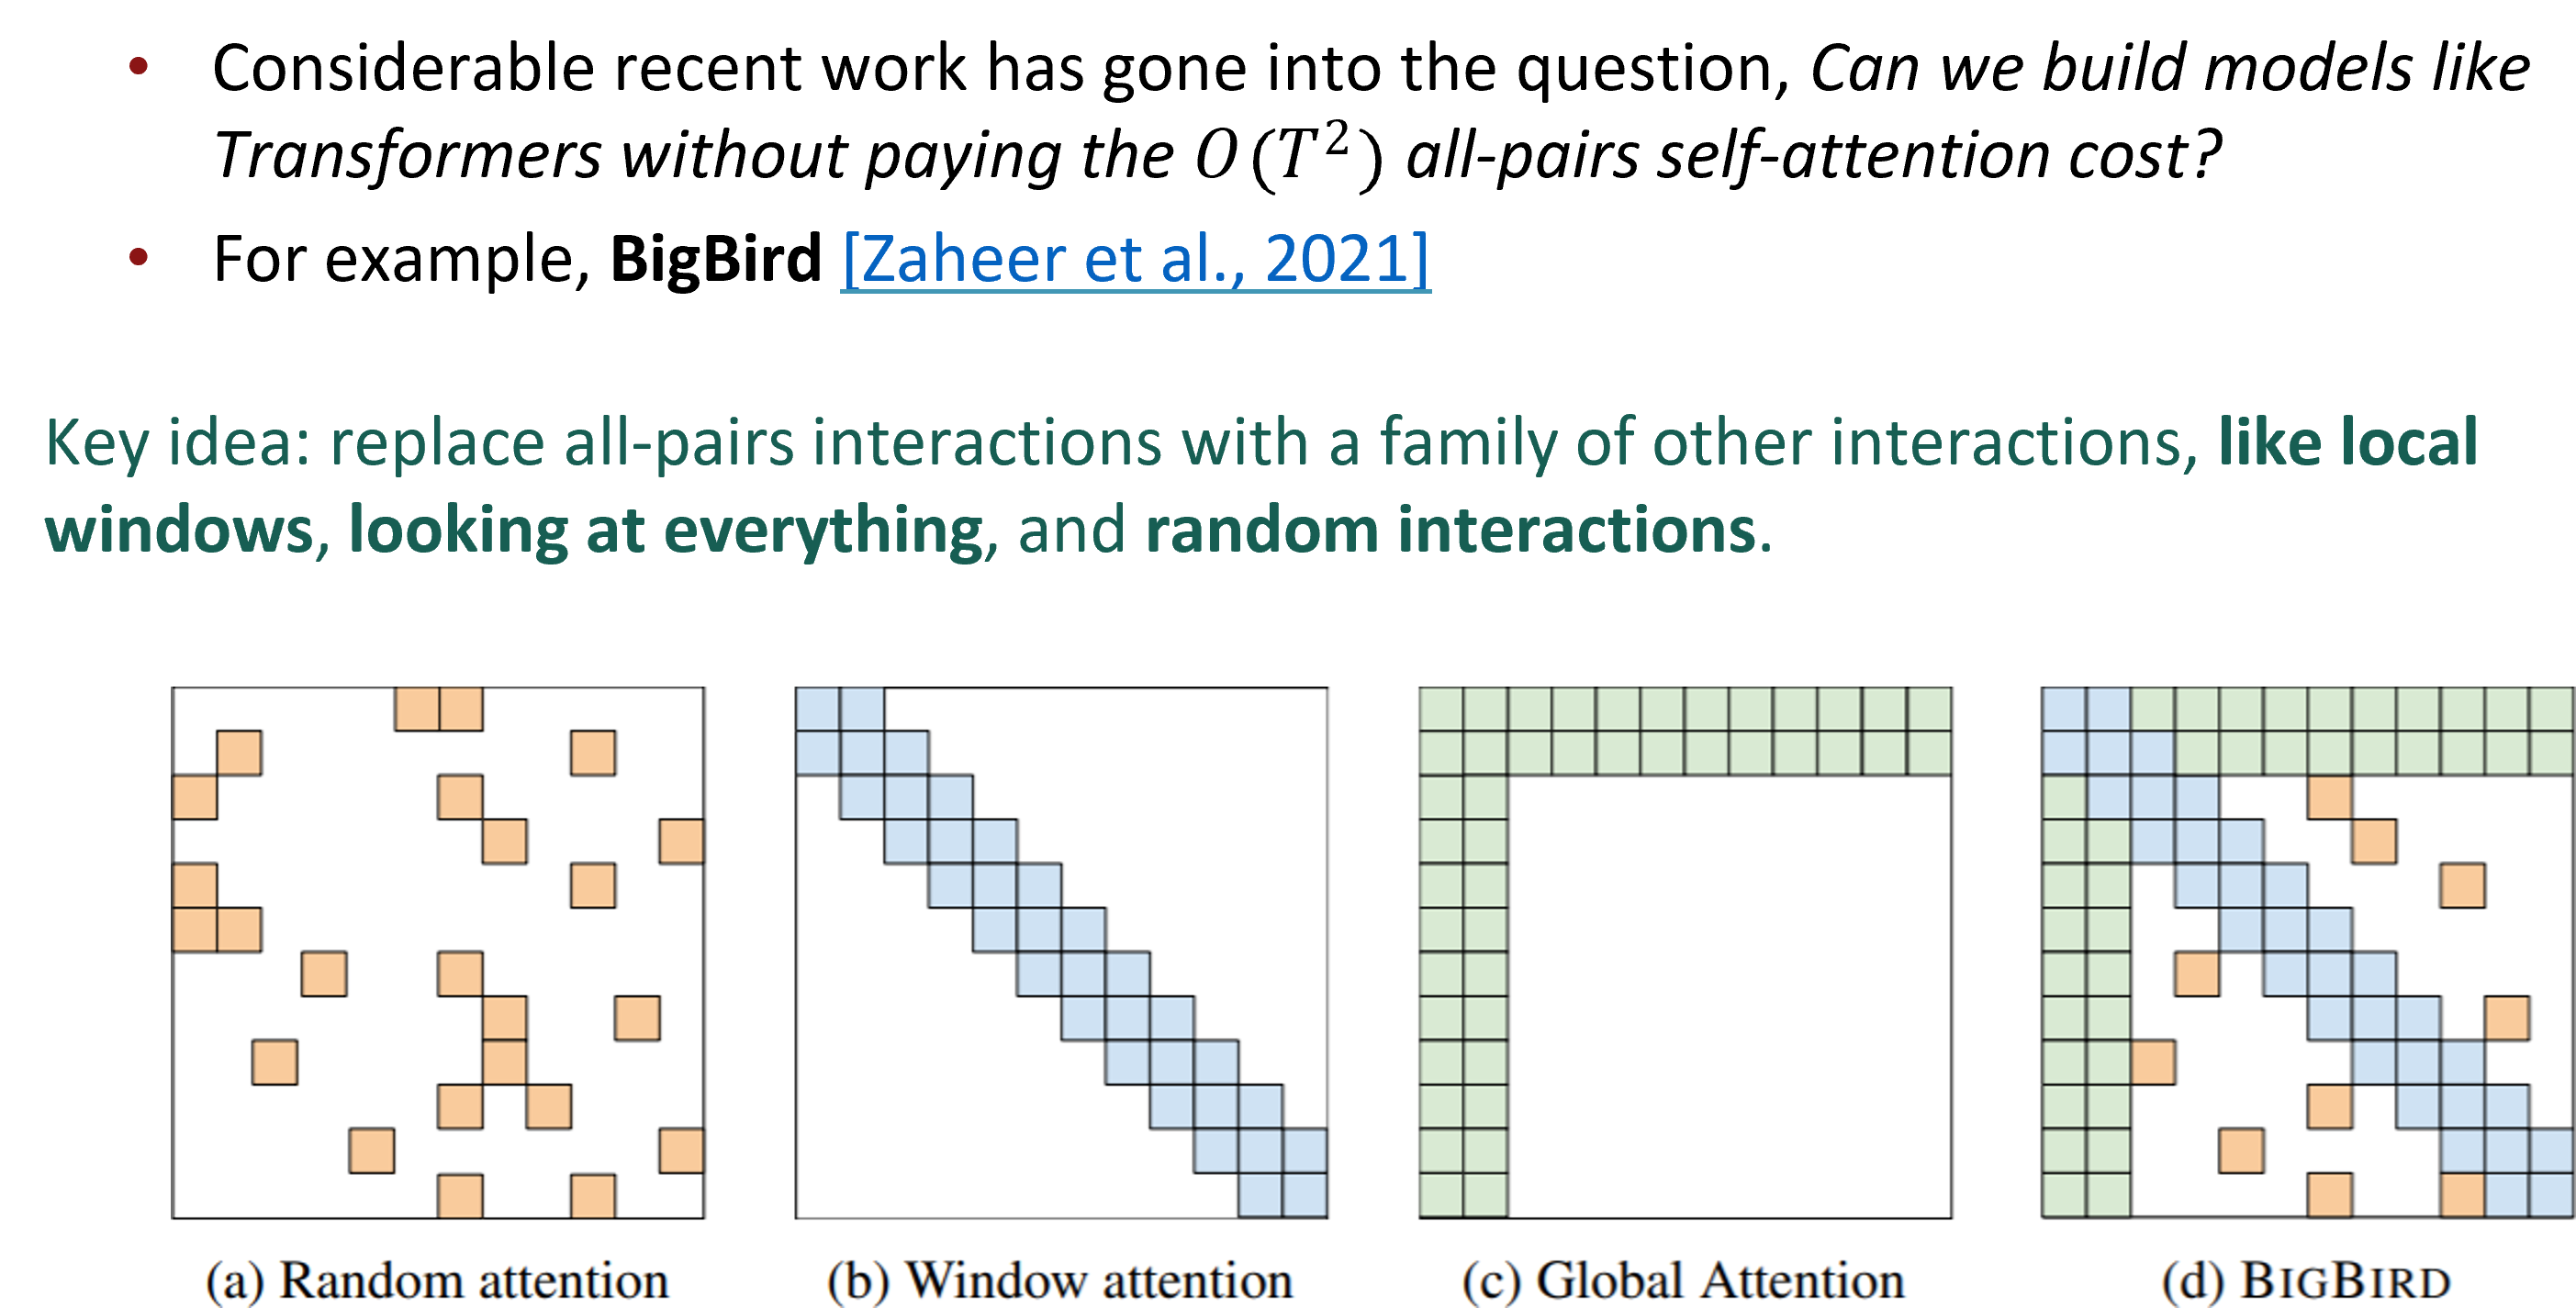
\includegraphics[width=\linewidth,keepaspectratio]{bert94}
			% \end{center}		
			
			% % {\tiny (Ref: John Hewitt)}

% \end{frame}

% %%%%%%%%%%%%%%%%%%%%%%%%%%%%%%%%%%%%%%%%%%%%%%%%%%%%%%%%%%%
% \begin{frame}[fragile]\frametitle{Recent work on improving on quadratic self-attention cost}

			
			% \begin{center}
			% 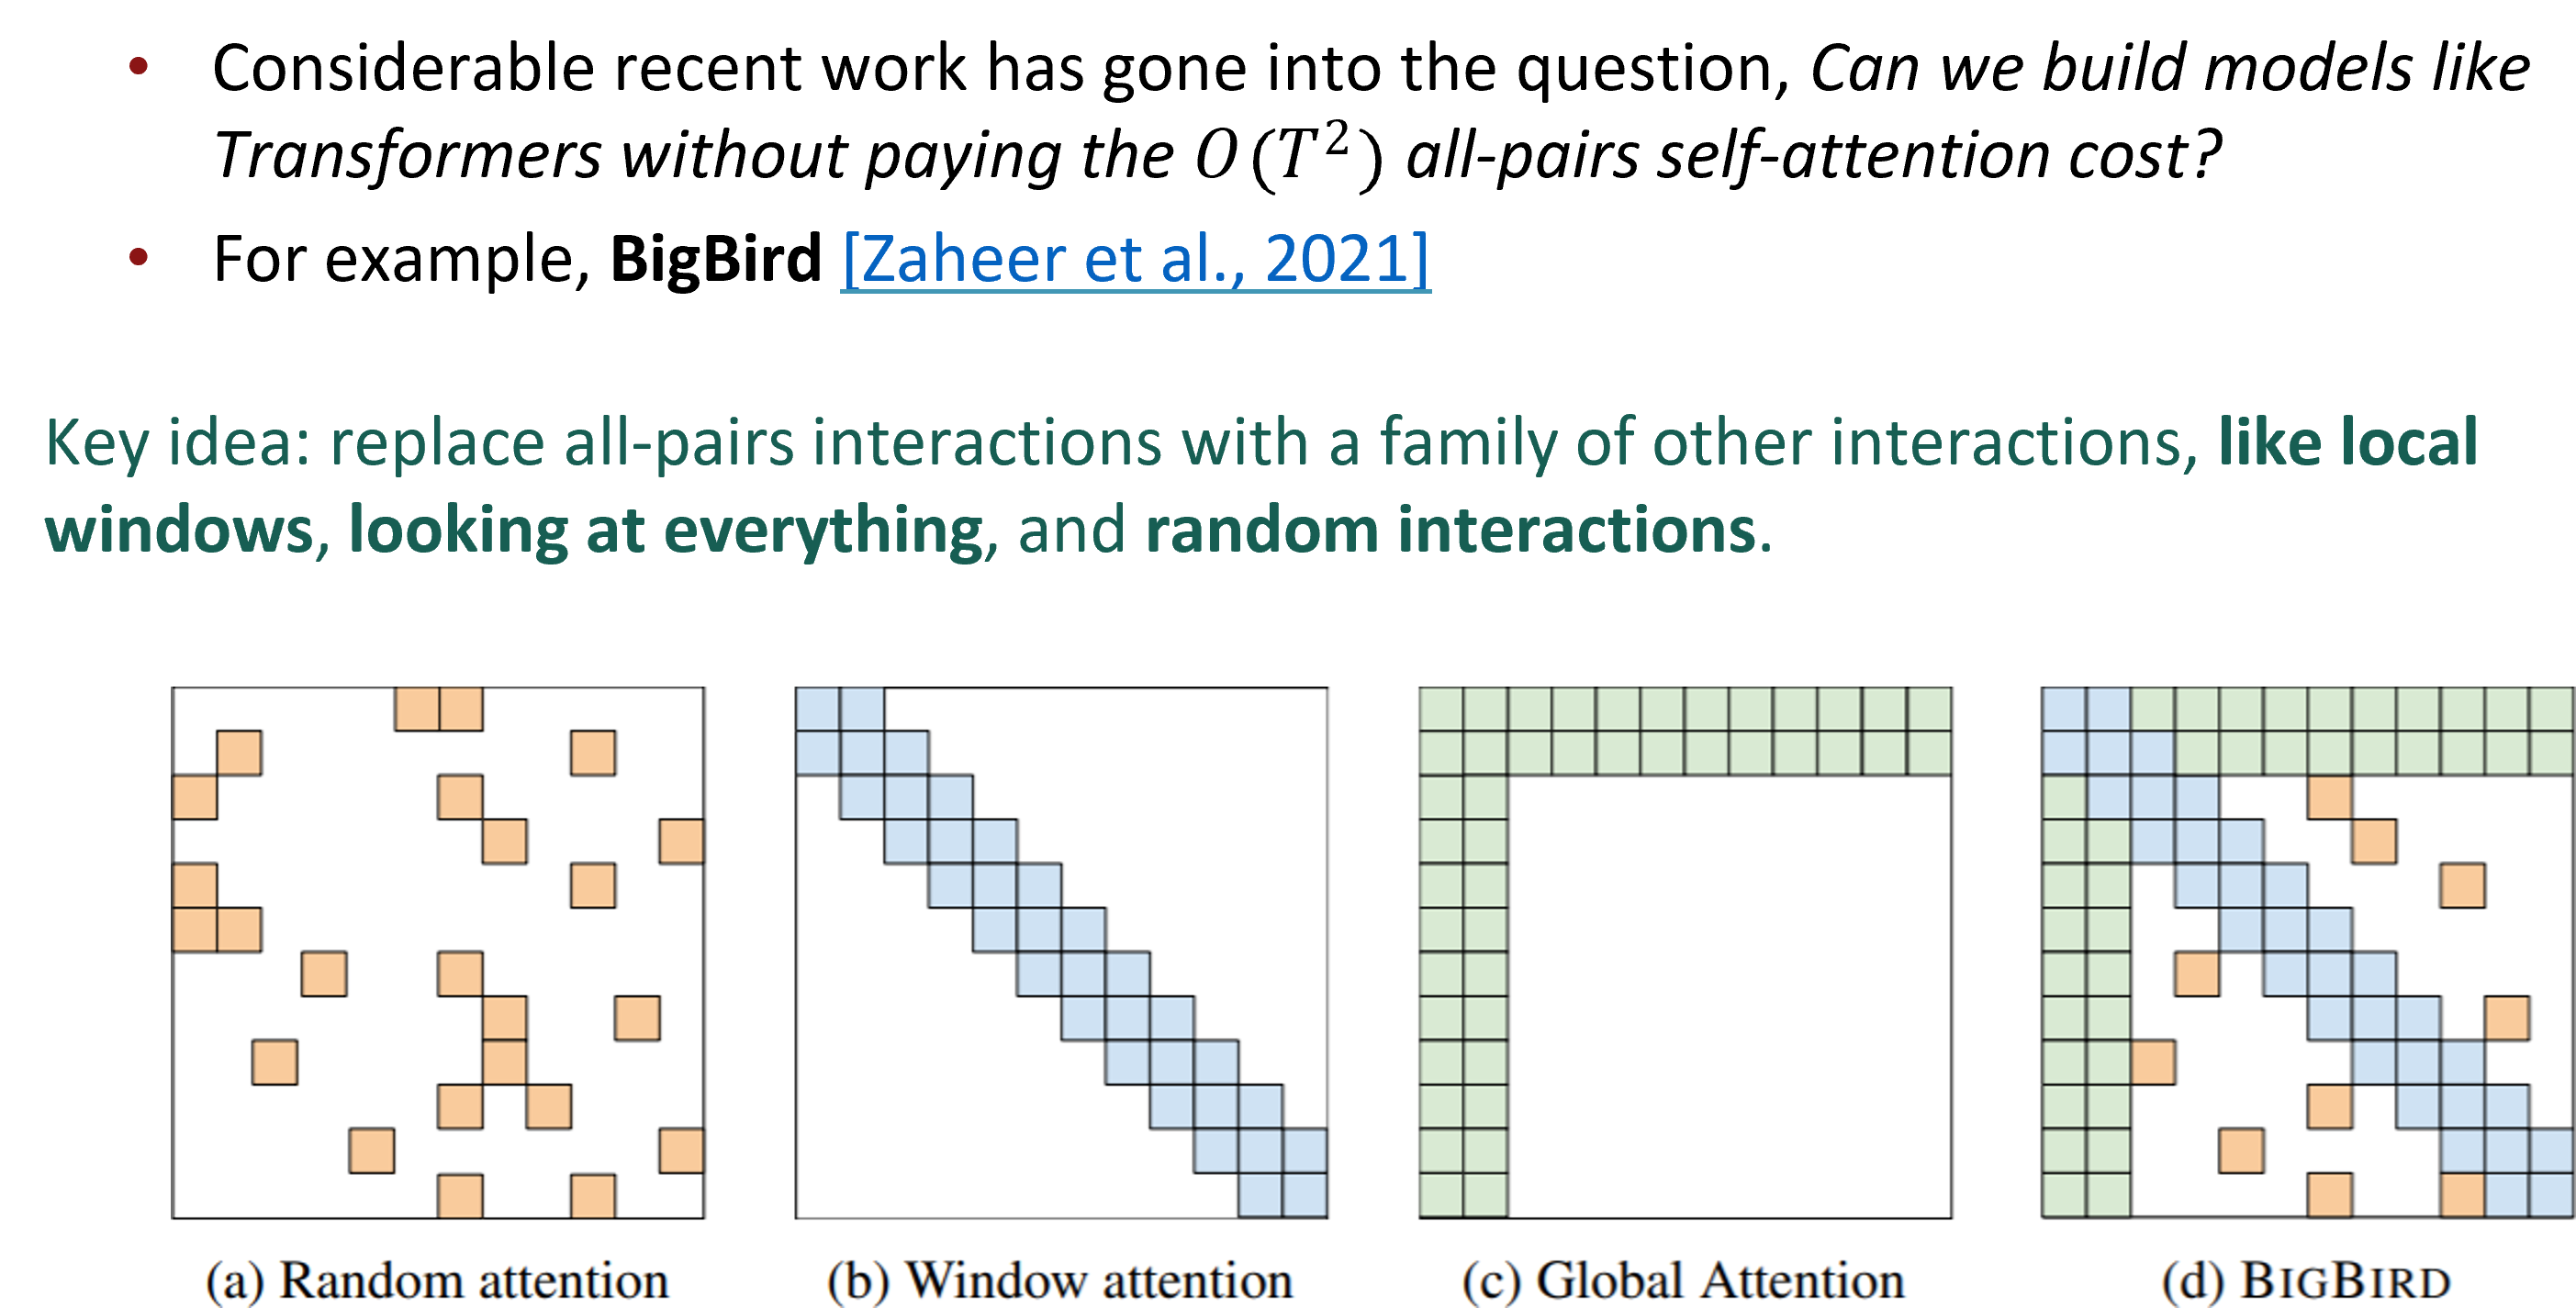
\includegraphics[width=\linewidth,keepaspectratio]{bert95}
			% \end{center}		
			
			% % {\tiny (Ref: John Hewitt)}

% \end{frame}



